\documentclass[12pt, oneside]{_praca_dyplomowa}

% rozmiar marginesów
\usepackage[a4paper, left=3.5cm, right=2cm, bottom=2.5cm, top=3cm]{geometry}
% zmieniony margines dla stron parzystych (druk dwustronny):
%\usepackage[a4paper, left=2cm, right=3.5cm, bottom=2.5cm, top=3cm]{geometry}
%\usepackage{times}
%\usepackage[default, none]{oxford}
%\usepackage{chicago}
% polskie znaki
\usepackage{setspace}
\usepackage{amsmath}
%\usepackage{graphs}

\usepackage[english]{babel}
%\usepackage[OT4]{polski}
\usepackage[T1]{fontenc}
%\usepackage[MeX]{polski}
\usepackage[utf8]{inputenc}

%\usepackage[pausing]{tracefnt}

% rysunki w formacie EPS
\usepackage[pdftex]{color,graphicx}
\usepackage{graphicx}
\usepackage{epsfig}
\graphicspath{{figures/}}
\usepackage[pausing]{tracefnt}
\usepackage{indentfirst} % akapit w pierwszej linii
\usepackage{color}
\definecolor{listing}{rgb}{0.1,0.3,0.3}
\usepackage{hyperref}
\hypersetup{
	unicode=true,
	pdftitle={Praca dyplomowa},
	pdfauthor={Sergiusz Urbaniak},
	pdfsubject={},
	pdfborder={0 0 0},
	pdfstartview=FitB,
	pdflang=pl,
	pdfdisplaydoctitle=true,
	plainpages=false
}
\usepackage{rotating}
\usepackage{import}
\usepackage{algorithmic}
\usepackage{algorithm}

\usepackage{listings}
\lstset{basicstyle=\small\ttfamily}

\usepackage{pdfpages}
\usepackage{url}

\usepackage{tikz}
\usetikzlibrary{mindmap,trees}

\usepackage{wrapfig}

%\fontsize{10}{12pt}
\providecommand{\abs}[1]{\lvert#1\rvert}

%INFORMACJA O PRACY
%==================
\tytul{Communication algorithms and principles for a prototype of a wireless mesh network}
\engtitle{Communication algorithms and principles for a prototype of a wireless mesh network}
\autor{Sergiusz Urbaniak}
\opiekun{dr inż. Remigiusz Olejnik}
\rok{2011}
\slowa{rf12b, rfm12b, hoperf, avr, atmega16, topologia kratowa, sieæ}
\opis{Description}
\kwords{}
\describe{Description}
\sloppy

\begin{document}

%\renewcommand\tablename{Tabela}
%\renewcommand\figurename{Rys.}

\begin{titlepage}

 \centering
  %\hbox{}
  \vfill                          
    { \large
        Z A C H O D N I O P O M O R S K I  \hspace{0.3 cm}  U N I W E R S Y T E T \\ 
        \vspace{0.2cm}
        T E C H N O L O G I C Z N Y \hspace{0.3 cm} W \hspace{0.3 cm} S Z C Z E C I N I E    } \\
    \vspace{1.cm}
   \epsfig{file={logowi.jpg},width=7 cm}
   \\ 


    \vspace{2.0 cm}

      \huge \textbf{PRACA DYPLOMOWA}\\ 

  \vspace{3.cm}                   
     { \huge \Tytul}\\ 
  


\begin{flushleft}
  \vspace{2.7 cm}
  {\large
  
 
        \hspace{7.0 cm}    Autor: \\
        \hspace{7.0 cm}    \Autor \\
  }

 \vspace{1.2 cm}

  {\large
        \hspace{7.0 cm}     Opiekun pracy: \\
        \hspace{7.0 cm}     \Opiekun \\
  }
\end{flushleft}

   \vspace{1.5 cm}
   {\large \Rok}
   \vfill                         
\end{titlepage}

\setstretch{1.6}
\chapter*{}

\vspace{1 cm}
\begin{center}                        
\LARGE{ \bf{Oświadczenie}} \\
\end{center}
Oświadczam, że przedkładaną prac magisterską/inżynierską kończącą studia napisałem samodzielnie. Oznacza to, że przy pisaniu pracy poza niezbędnymi konsultacjami, nie korzystałem z pomocy innych osób, a w szczególności nie zlecałem opracowania rozprawy lub jej części innym osobom, ani nie odpisywałem rozprawy lub jej części od innych osób. Potwierdzam też zgodność wersji papierowej i elektronicznej złożonej pracy. Mam świadomość, że poświadczenie nieprawdy będzie w tym przypadku skutkowało cofnięciem decyzji o wydaniu dyplomu.
\vspace{3.0cm}
\begin{flushleft}
\hspace{10.0 cm}     Sergiusz Urbaniak\\
\end{flushleft}

\normalsize

\tableofcontents
\listoffigures
%\renewcommand\listtablename{Spis tabel} 
\listoftables
\chapter{Introduction}% {{{1

\begin{figure}[H]
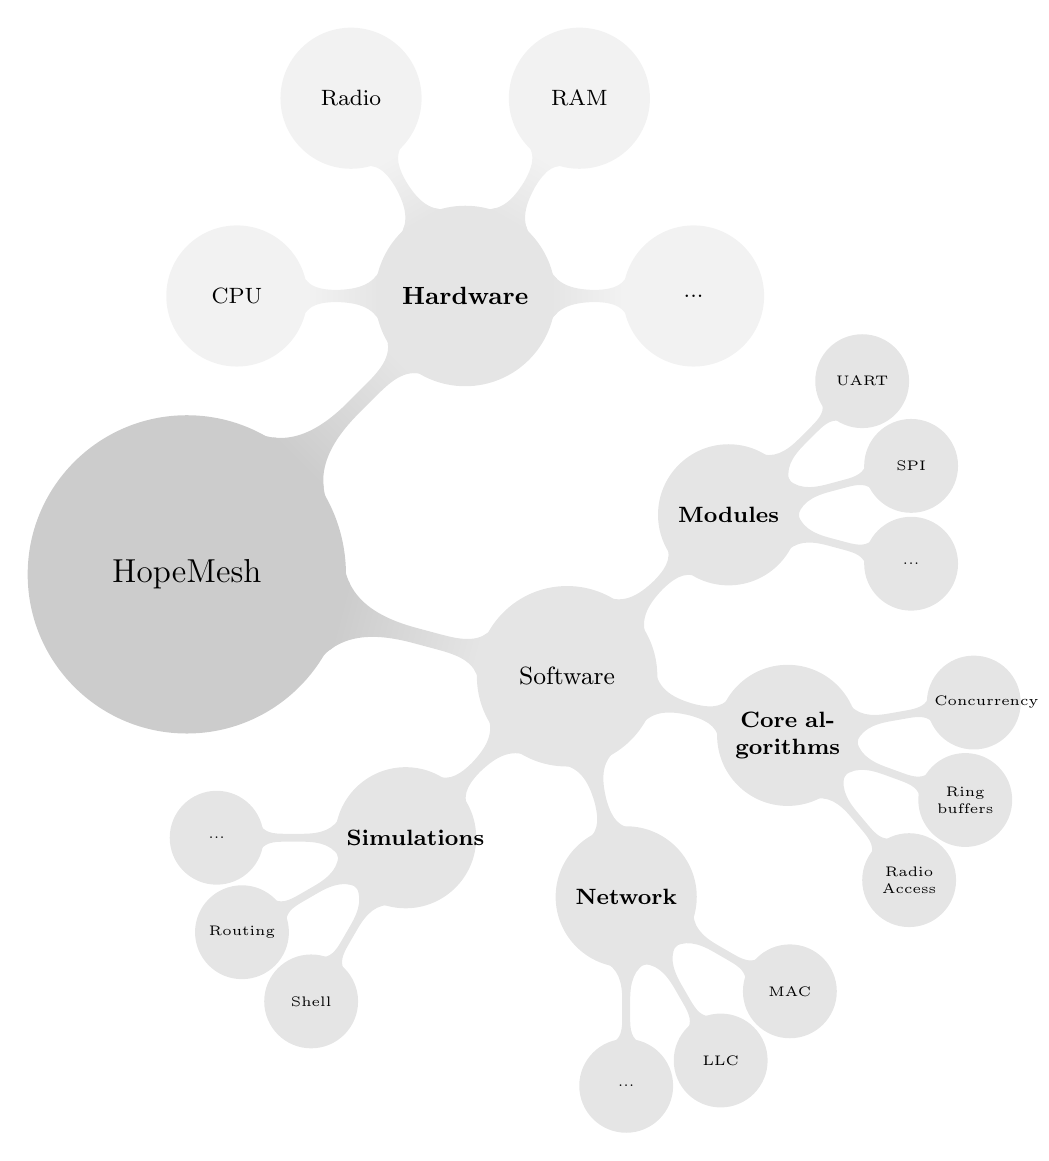
\begin{tikzpicture}
\path[mindmap, concept color=lightgray!80]
    node[concept] {HopeMesh}
    [clockwise from=45]
    child[concept color=lightgray!40] {node[concept] {\textbf{Hardware}}
        [clockwise from=180]
        child[concept color=lightgray!20] {node[concept] {CPU}}
        child[concept color=lightgray!20] {node[concept] {Radio}}
        child[concept color=lightgray!20] {node[concept] {RAM}}
        child[concept color=lightgray!20] {node[concept] {...}}
    }
    child[concept color=lightgray!40] {node[concept] {Software}
        child {node[concept] {\textbf{Modules}}
            child {node[concept] {UART}}
            child {node[concept] {SPI}}
            child {node[concept] {...}}
        }
        child {node[concept] {\textbf{Core algorithms}}
            [clockwise from=10]
            child {node[concept] {Concurrency}}
            child {node[concept] {Ring buffers}}
            child {node[concept] {Radio Access}}
        }
        child {node[concept] {\textbf{Network}}
            [clockwise from=330]
            child {node[concept] {MAC}}
            child {node[concept] {LLC}}
            child {node[concept] {...}}
        }
        child {node[concept] {\textbf{Simulations}}
            [clockwise from=240]
            child {node[concept] {Shell}}
            child {node[concept] {Routing}}
            child {node[concept] {...}}
        }
    }
    ;
\end{tikzpicture}
\caption{HopeMesh project mind map}
\label{fig:mindmap}
\end{figure}

This thesis has the goal to implement an advanced and refined version of the predecessor implementation \cite{korniowski} for a fail-safe mesh network prototype using embedded technologies. The project name "HopeMesh" reflects the major goal to implement a mesh routing algorithm based on cheap HOPERF radio modules. This goal can be split in the following aspects according to the mind map as seen in figure \ref{fig:mindmap}:
\begin{itemize}
    \item \textbf{Hardware: } The goal is to explore alternative, enhanced and reusable hardware solutions for an embedded implementation.
    \item \textbf{Modules:} The goal is to find the necessary software modules from an abstract architectural point of view.
    \item \textbf{Algorithms:} The goal is to explore and elaborate on concrete algorithms and data structures for the implementation of the software modules.
    \item \textbf{Network:} The goal is to implement a network stack which not only provides a mesh routing based on the B.A.T.M.A.N. algorithm but also provides a real network stack.
    \item \textbf{Simulation :} The goal is to provide the basis for a simulation environment for the provided algorithms that can execute on regular PCs.
\end{itemize}

The author wants to prove that an implementation of a robust and scalable mesh network using embedded devices despite its hardware constraints is quite possible. He wants to explore algorithms and software architectures usually hidden behind the curtain of operating systems.
The desired end result is not only to have a working mesh network prototype but also an algorithmic framework for further development. Therefore the author also wanted to provide a framework which allows to try and research future algorithms on a regular PC.
Finally the author wanted to provide a reproducible hardware design in order to able to equip a complete laboratory of mesh nodes for further research and investigation.

\section{Thesis overview}% {{{2
The thesis is structured in the same order as the above mentioned goals. The first part analyzes the existing prototype hardware. An enhanced version is proposed by providing an alternative CPU and the connection of external RAM. Level shifters are introduced for the connection of the RFM12B radio module and the existing UART connection is being enhanced by an USB interface. Finally connectors for an external keyboard and an external LCD module are introduced.

The second part elaborates on the envisioned software architecture. It identifies the necessary software modules which have to be implemented in order to provide a robust design. It defines modules for the human interaction and for the internal state control. The network stack module and the RFM12B driver module are identified for the mesh network access.

The third part explores the algorithmic foundations and data structures which are being used for the implementation. Different concurrency models are being analyzed and a threading framework for the software modules is proposed. An algorithm for the seamless integration of the UART module is being proposed and finally the complex concurrency behavior of the RFM12B driver module analyzed.
The fourth part is solely dedicated to the network stack. The implemented network layers and packet structures are described as well the used transmission encoding.

The last part elaborates on the implemented simulations in order to verify the modeled algorithms, data structures and network stacks on a regular PC.

\chapter{Hardware Design}% {{{1
\section{Hardware Modules}% {{{2
\subsection{CPU} % {{{3
\label{sub:cpu}
The predecessor implementation uses an Atmel Atmega16 RISC microprocessor implementing the harvard architecture. The author decided to analyze whether this CPU is still adequate for the new implementation. The author set up the following requirements for the new hardware architecture:

\begin{itemize}
    \item \textbf{GCC tool chain:} The author wanted to use an open source development environment using the C language. The existing GCC tool chain is known to most programmers and the compiler can be used cross-platform on Windows, the MacOS and Linux operating systems.
    \item \textbf{Extensibility:} The author wanted to use a CPU which has the possibility to be extended with external hardware. Especially the author wanted to use a CPU which allowed to be extended with external RAM.
\end{itemize}

The result was a different CPU being used in this thesis, namely the Atmega162 and not the Atmega16 as in the predecessor thesis. The Atmega162 does not have ADC capabilities but is rather specialized on digital peripheral hardware. It has an external memory interface called XMEM which allows the connection of an external SRAM module. Furthermore it has more digital I/O pins available than the Atmega16.

\subsection{RAM}% {{{3
The CPU was connected with an external 62256 SRAM \cite{62256-datasheet} chip using a register latch. It offers 32k external RAM. The configured RAM configuration is shown in figure \ref{fig:ram}. Since the CPU implements the harvard architecture no program space is available in the RAM.

\begin{figure}[H]
\centering
\import{figures/}{ram.pdf_tex}
\caption{RAM configuration}
\label{fig:ram}
\end{figure}

The following memory data sections were configured:

\begin{itemize}
    \item \textbf{Register Memory space (256 Bytes):} This memory space is constant. It contains internal registers.
    \item \textbf{Stack in internal SRAM (1,024 Bytes):} This memory space is solely used for the stack. In the predecessor thesis \cite{korniowski} this memory space also held static data and the heap.
    \item \textbf{Data section in external SRAM (1,544 Bytes):} This newly available memory space is used for static data. This data section was measured by listing the symbols of the final binary using the "avr-nm" program and differs depending on the usage of static variables in the program.
    \item \textbf{Heap section in external SRAM (31,223 Bytes):} This newly available memory space is used for the heap. It depends on the size of the data section.
\end{itemize}

One can see that the external RAM configuration was desperately needed. The new thesis implementation uses more than 1K of static variable space which already exceeds the available native CPU memory. With the usage of external RAM a total of nearly 32K heap RAM is available not including static variables. Furthermore the complete (and efficient) internal RAM is used solely for the runtime stack.

One entry in the network routing table (see chapter \ref{sec:route}) needs of a total 11 bytes. With the current RAM configuration therefore a maximum number of 2,838 nodes can be addressed if no other data is stored on the heap.

\section{Schematic}% {{{2
The predecessor thesis \cite{korniowski} connected the RFM12B radio module directly to the CPU. The consequence is an operating voltage of 5V for the radio module which is out of specification. The maximum operating voltage for the radio module is 3.3V. Therefore the author connected the radio module using level shifters \cite{schutte}.

Furthermore the nowadays nearly deprecated RS-232 connection was replaced with an USB connection. The USB driver was migrated from the AVR-CDC \cite{avrcdc} project. It uses an AVR Attiny2323 processor in order to simulate a low-speed USB stack. The CDC protocol has native support in Linux (using a kernel version >2.6.31) but a Windows driver is available on the project site \cite{avrcdc}.

Finally the author placed PS/2 keyboard and HD4780 LCD connectors for future enhancements.

The complete schematic of the HopeMesh hardware is shown on the next two following pages.

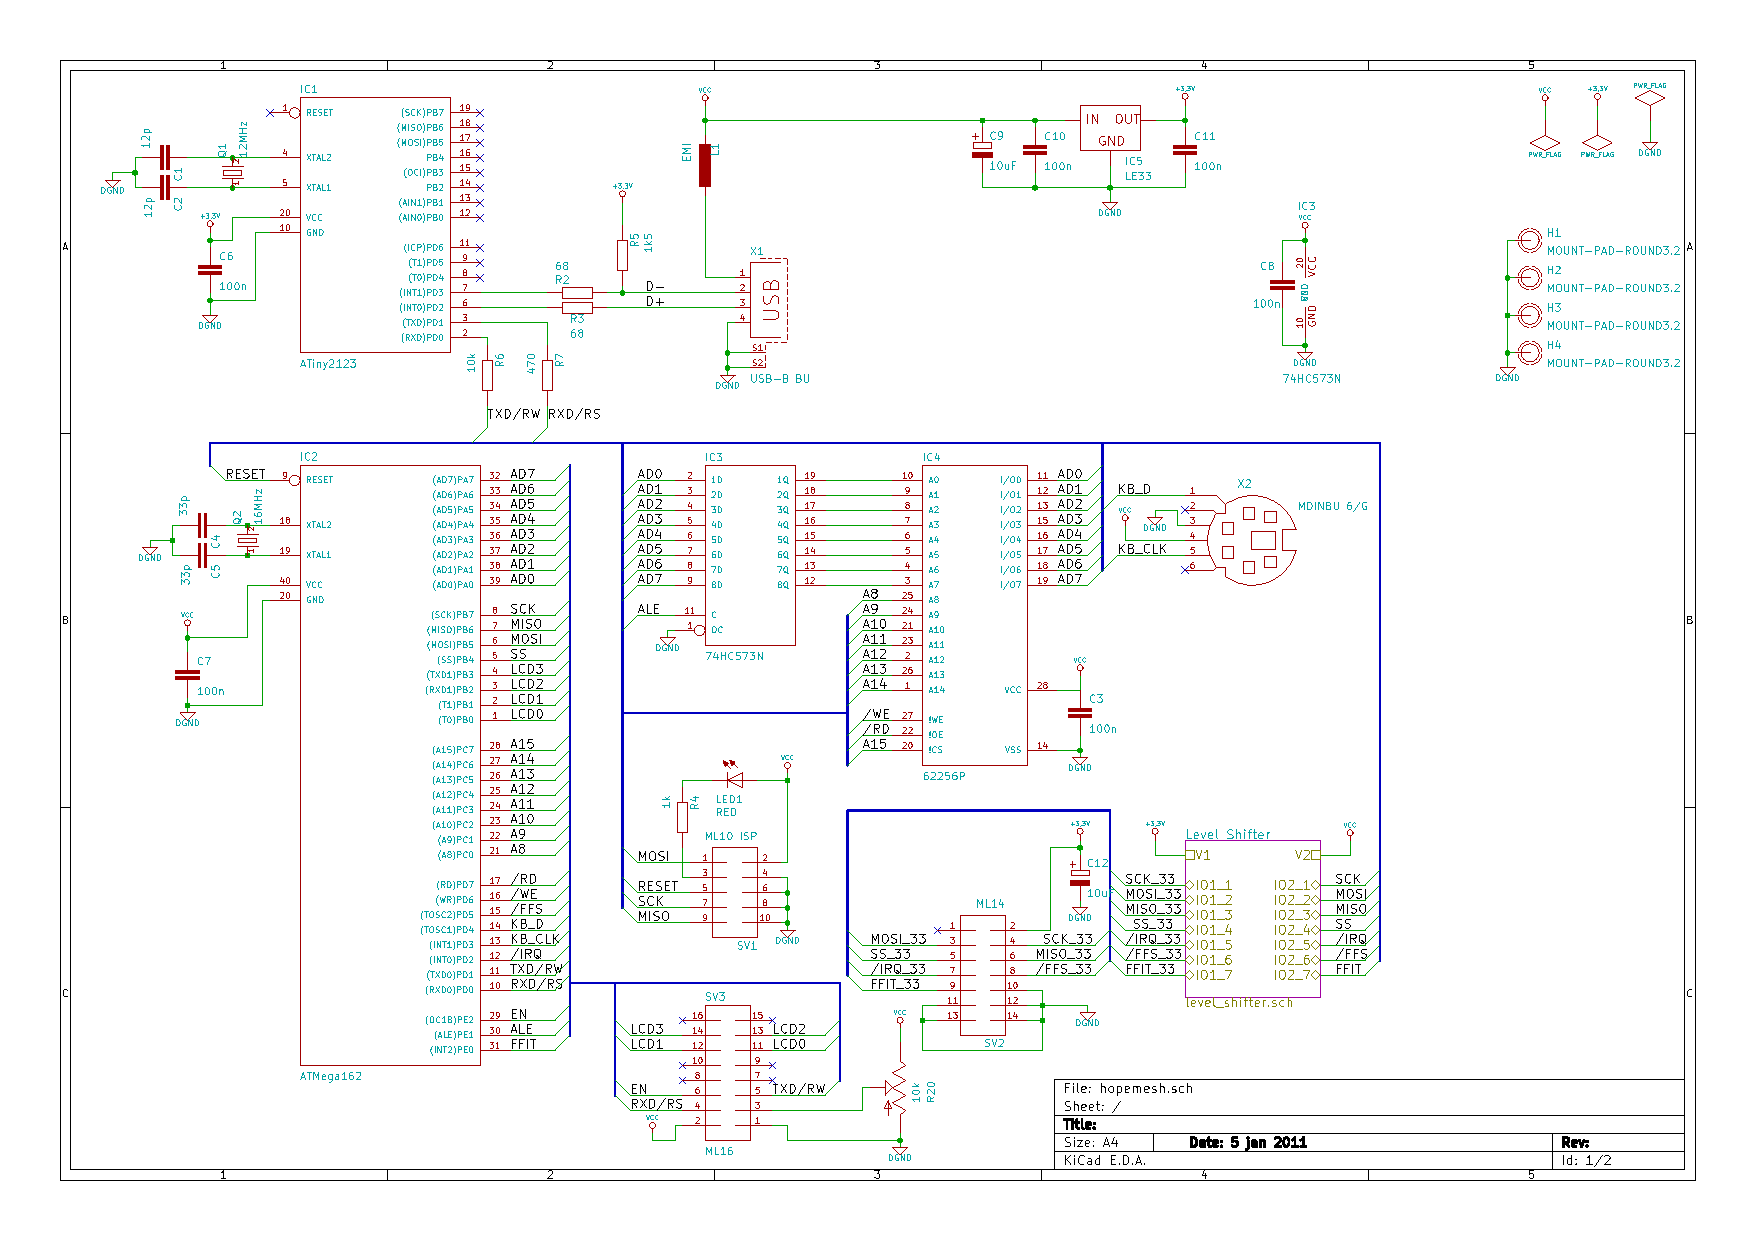
\includepdf[
    landscape,
    addtolist={
        1,
        figure,
        HopeMesh schematic,
        fig:hopemesh-sch
    }
]{figures/hopemesh-sch.pdf}

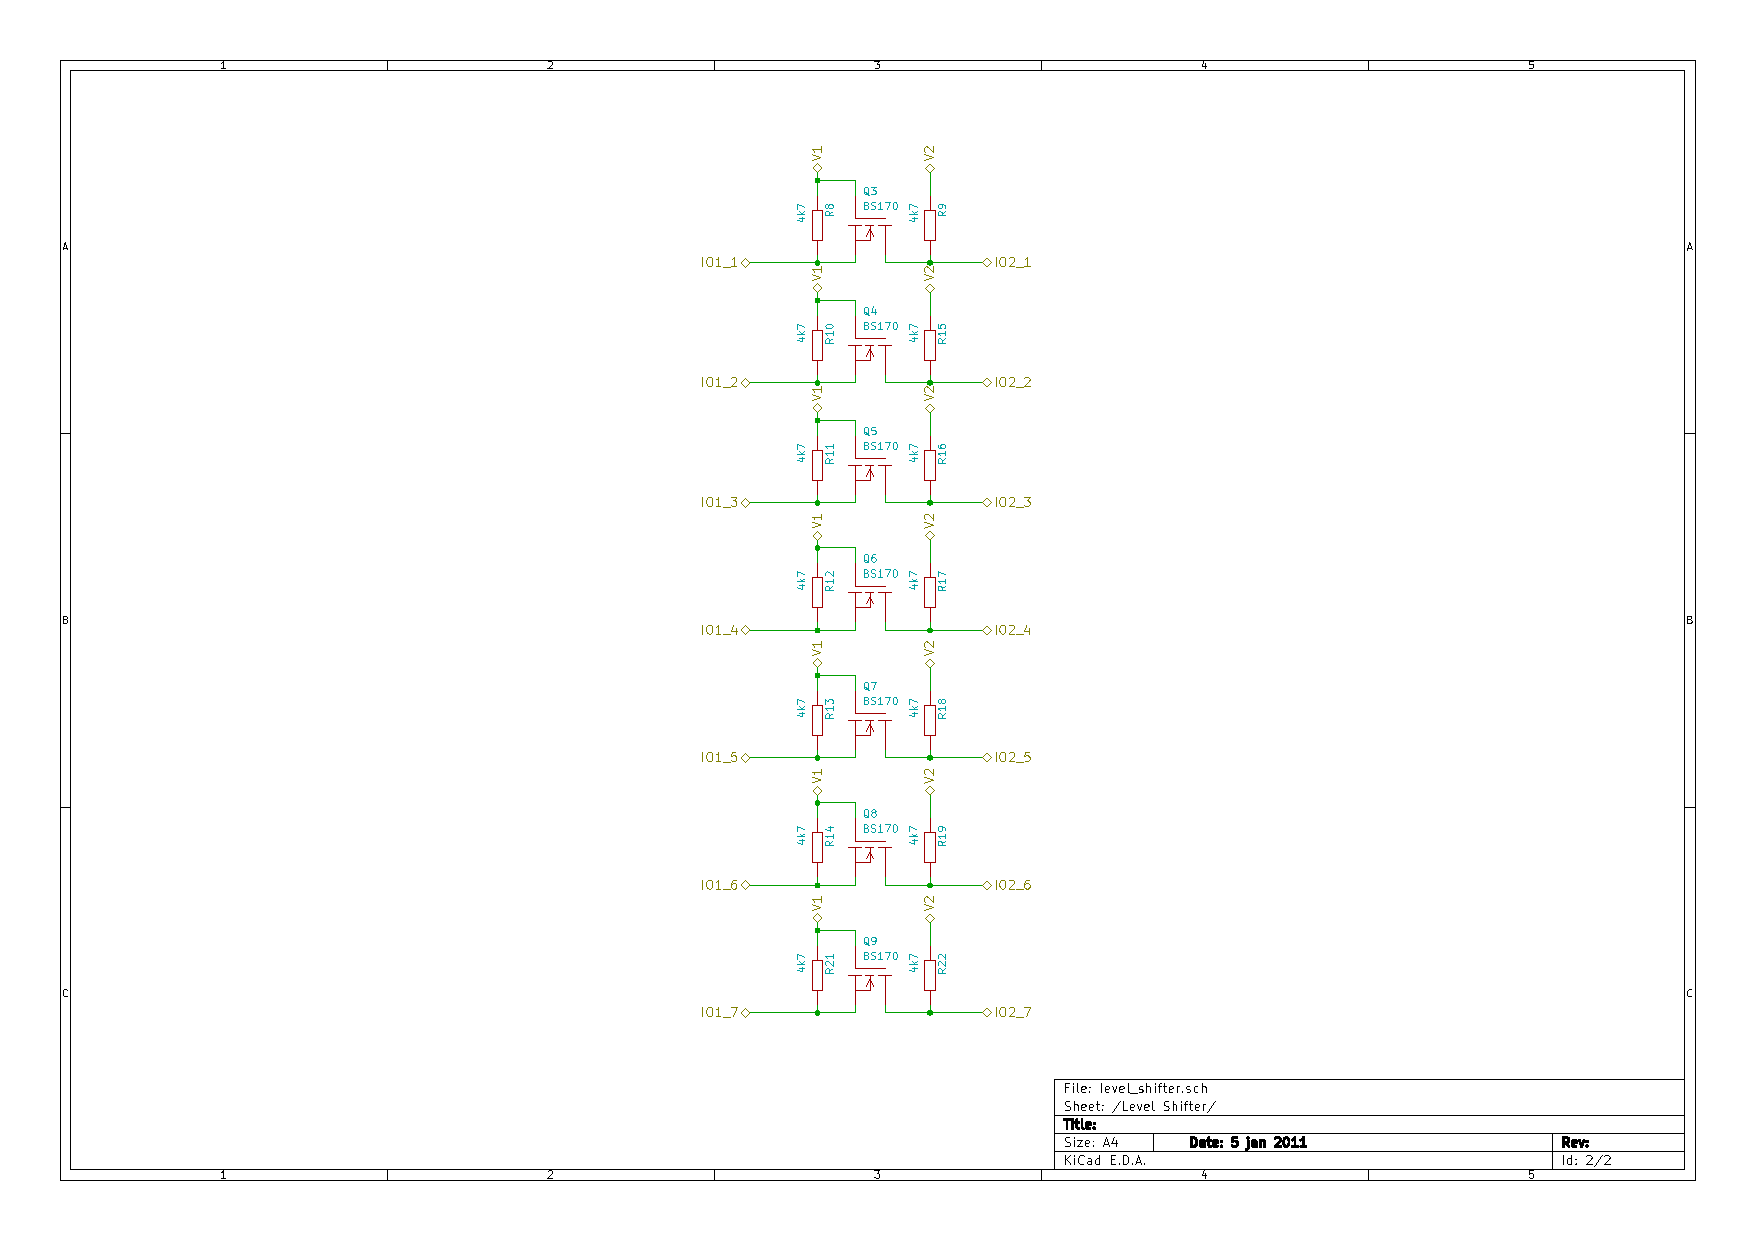
\includepdf[
    landscape,
    addtolist={
        1,
        figure,
        HopeMesh level shifter schematic,
        fig:hopemesh-sch-levelshifter
    }
]{figures/hopemesh-sch-levelshifter.pdf}

\section{Printed Circuit Board}% {{{2
\begin{figure}[H]
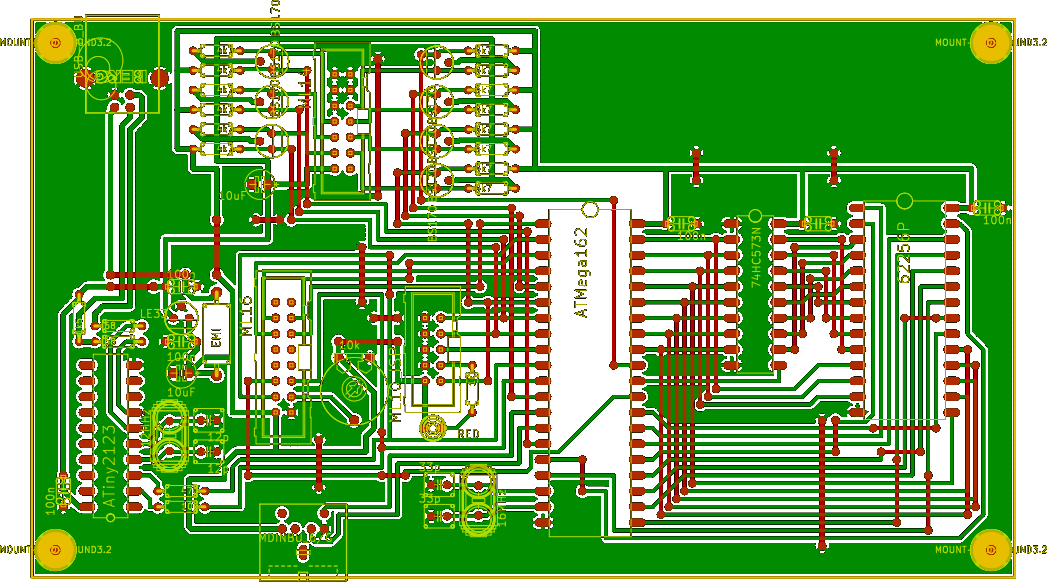
\includegraphics[width=\textwidth]{figures/2nd_rev_pcb_layout.png}
\caption{2nd revision PCB layout}
\end{figure}

In order to able to set up future mesh nodes a reproducible hardware design had to designed. The goal was to be able to produce many mesh nodes and to be able to equip a whole laboratory. One possibility is to manually wire each mesh node. Due to the complexity of the schematic this solution was not acceptable. The author decided to design a printed circuit board (PCB) in order to be able to produce new mesh nodes quickly. The following design requirements were established by the author:

\begin{itemize}
    \item \textbf{One sided PCB: } The PCB was aimed to be manufactured in an uncomplicated environment. Two-sided PCBs allow minimizing the physical size of the device but for research this is not an important requirement. On the other hand two-sided PCBs require additional effort. Through-holes have to be manufactured and eventually the upper side of the PCB has to be laminated in order to prevent shorts.
    \item \textbf{Non-SMD parts: } The author explicitly avoided SMD parts. The goal was to be able to solder the parts manually with commonly available electronic parts.
\end{itemize}

The actual design of the PCB (Printed Circuit Board) was performed in three iterative phases:
\begin{itemize}
    \item \textbf{Manually wired prototype :} In order to have a proof of concept a first working prototype was constructed by the author manually. This board was not used for the final realization but was used in order to test the external RAM as well as the UART-USB connection.
    \item \textbf{1st revision PCB :} A first revision of the PCB was designed and manufactured. Despite a function node a few design improvements were identified. The trace count and surface mounting the existing resistors were identified as a further improvement.
    \item \textbf{2nd revision PCB :} The final revision of the PCB was designed in smaller dimensions and the design flaws from the first revision were corrected.
\end{itemize}

\begin{figure}[H]
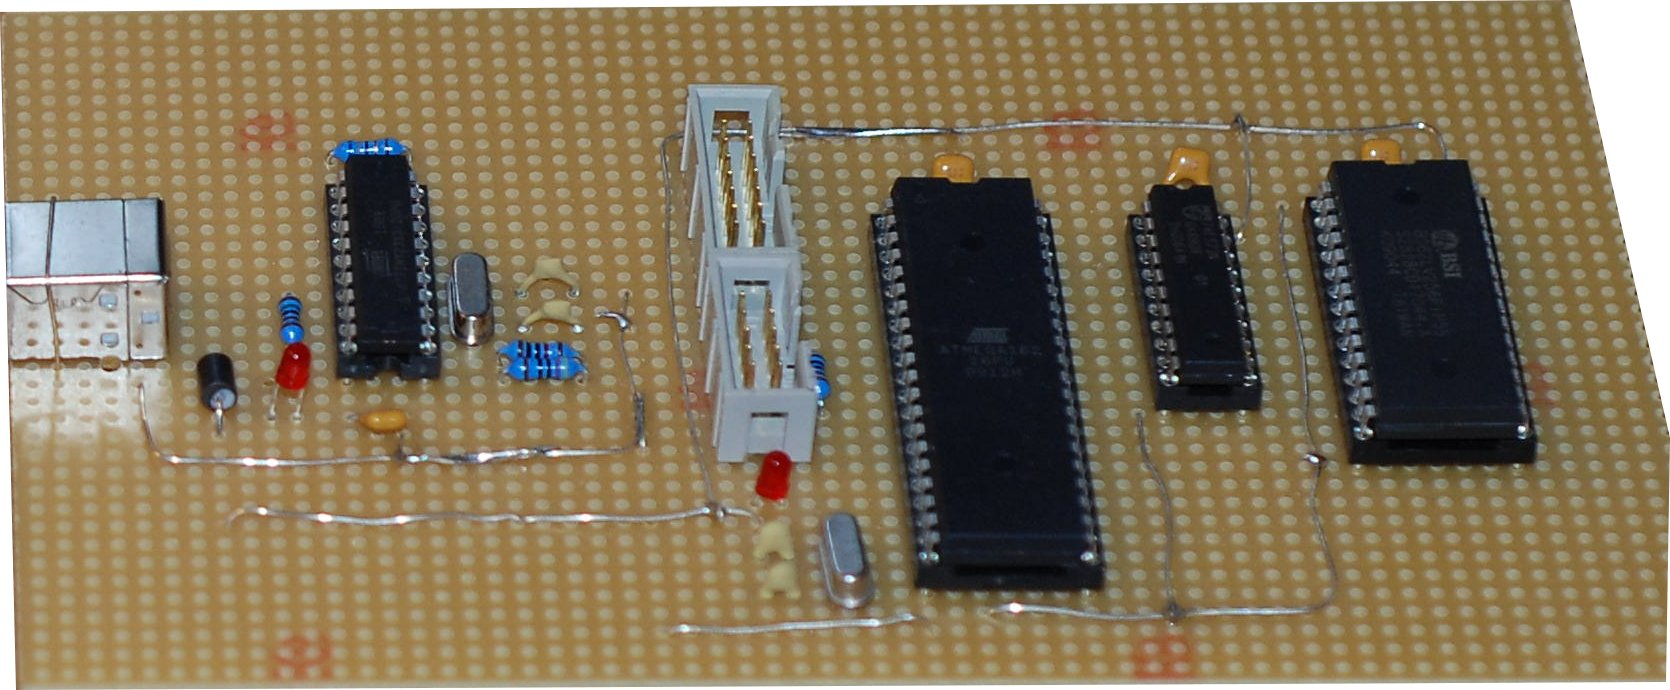
\includegraphics[width=\textwidth]{figures/prototype_pcb.jpg}
\caption{Manually wired prototype board}
\end{figure}

The final version of the PCB was carefully designed to have a logical and effective layout of components. Figure \ref{fig:2ndrev_pcb} shows the zones which include the different hardware modules. The following zones were designed:

\begin{figure}[H]
    \centering
    \import{figures/}{2nd_rev_pcb.pdf_tex}
    \caption{2nd revision PCB areas}
    \label{fig:2ndrev_pcb}
\end{figure}

\begin{itemize}
    \item \textbf{USB: } The USB parts and connectors are being placed in this zone. In order to have a comfortable connection to the cable the USB connector was placed in the left upper corner.
    \item \textbf{Power supply: } Right next to the USB zone the PSU parts are placed.
    \item \textbf{RFM12B: } The radio modules as well as the level shifters were placed next to each other.
    \item \textbf{ISP: } The In-System-Programmer connector was placed next to the CPU in order to reduce scattering effects.
    \item \textbf{CPU, Latch \& SRAM: } These chips were placed next to each other in order to reduce the bus trace lengths as much as possible.
\end{itemize}

\chapter{Software modules and algorithms}% {{{1
\section{Module architecture} % {{{2
\label{sec:module_architecture}

\begin{figure}[H]
\centering
\import{figures/}{modules_component_diagram.pdf_tex}
\caption{Software modules (UML 2.0 component diagram)}
\label{fig:modules}
\end{figure}

The author chose a top-down design approach for the software part of the thesis implementation. This approach consists the following steps:

\begin{enumerate}
    \item Design a general architecture and identify the necessary software parts (modules) which need to be connected together.
    \item Research the necessary abstractions how the plumbing and inner interoperability actually should work.
    \item Research the necessary algorithms for the final implementation.
\end{enumerate}

The following chapters reflect the above described approach. Figure \ref{fig:modules} shows the general module architecture of the thesis implementation. First the following module stereotypes were identified for the complete software stack:

\begin{itemize}
    \item \textbf{Userspace modules:} Act like regular "programs". They interact with the user, retrieve user input and generate user output.
    \item \textbf{Driver modules:} Provide the necessary abstractions and APIs to external or CPU internal hardware.
    \item \textbf{Daemon modules:} These modules are similar to userspace modules but run in the background only. They do not interact with the user.
    \item \textbf{Library modules:} Implement APIs and provide those to userspace or daemon modules.
\end{itemize}

Afterwards the following concrete modules were identified and implemented by the author:

\begin{enumerate}
    \item \textbf{UART \emph{<<driver>>}:} This driver module is responsible for the UART interface. It implements an optimized UART access using ring buffers.
    \item \textbf{SPI \emph{<<driver>>}:} This driver provides the API to access the serial peripheral interface.
    \item \textbf{RFM12 \emph{<<driver>>}:} Implements the API to access the RFM12 hardware module. It uses the SPI driver module.
    \item \textbf{Timer \emph{<<driver>>}:} This driver provides the API and callbacks for timer services.
    \item \textbf{Network \emph{<<library>>}:} This libray module provides the complete network stack API to userspace modules.
    \item \textbf{Watchdog \emph{<<daemon>>}:} This daemon updates the watchdog timer of the CPU. Furthermore it provides an API in order to reset the CPU manually and add an error stack information stored in the EEPROM.
    \item \textbf{Clock \emph{<<daemon>>}:} This daemon is responsible to measure the current time. It uses the timer driver module.
    \item \textbf{Shell \emph{<<userspace>>}:} This userspace module is responsible for receiving commands from the serial UART driver, executing commands and printing the result back.
    \item \textbf{Receiver \emph{<<userspace>>}:} This userspace module prints out received messages using the UART driver module.
\end{enumerate}

\section{Module orchestration}% {{{2
Designing a software system that executes on embedded micro-controllers implies a lot of challenges when many software modules are involved and complexity grows. The conceptually defined modules must be somehow implemented. If the micro-controller lacks an operating system then there is no possibility of using provided abstractions and APIs for module orchestration and execution. Another challenge are limited hardware resources which prevent the deployment of many existing operating system kernels. Basically there are two types of execution models which can be implemented in micro-controllers:

\begin{enumerate}

\begin{figure}[H]
    \centering
    \import{figures/}{sequential_execution.pdf_tex}
    \caption{Sequential execution model}
\end{figure}

    \item \textbf{Sequential execution model:} This type sequentially executes all modules inside an infinite main loop starting from the first module until the last one. Once the last module ends the execution starts again from the first module.

\begin{figure}[H]
\centering
\import{figures/}{concurrent_execution.pdf_tex}
\caption{Concurrent execution model}
\end{figure}
    \item \textbf{Concurrent execution model:} This type executes modules concurrently. Instead of having an infinite main loop that iterates sequentially over all modules the main function only initializes and launches concurrent modules.
\end{enumerate}

\subsection{Sequential execution}% {{{3
This model does not necessarily needs operating system support or frameworks. It can be simply implemented as a sequence of function calls inside an infinite loop as shown in algorithm \ref{alg:sequential execution}.

\begin{algorithm}[H]
\caption{Sequential model algorithm}
\label{alg:sequential execution}
\begin{algorithmic}
\WHILE{$true$}
\STATE $module_1$
\STATE $module_2$
\STATE $...$
\STATE $module_n$
\ENDWHILE
\end{algorithmic}
\end{algorithm}

There is one challenge that comes with this type of execution model. That is that only one module can execute at a time due to its sequential nature. If a module i.e. waits for an external resource to provide data it must not block the execution of the main loop until the external resources becomes ready. This would prevent the execution of the other modules. The classic solution to this problem is the introduction of states in modules. Module states can be implemented as classical Finite State Machines \cite{booth}.

If we take the example from above about waiting for external resources a finite state machine for modules can be modeled as shown in figure \ref{fig:statemachine}.

\begin{figure}[H]
\centering
\import{figures/}{state_machine.pdf_tex}
\caption{State Machine for a module}
\label{fig:statemachine}
\end{figure}

State machine models can be implemented using \texttt{if} or \texttt{case} statements which is shown in algorithm \ref{alg:statemachine}. The nice side effect of a state machine based implementation is the non-blocking nature of the module execution. Take for instance the execution of state 1 "Waiting" as shown in figure \ref{fig:statemachine}. The CPU only needs to execute as many instructions as are necessary to check if the awaited resource is available. If the resource is not available the execution returns to the main loop and the next module (together with its state machine) is being executed.

\begin{algorithm}[H]
\caption{State machine algorithm}
\label{alg:statemachine}
\begin{algorithmic}
\IF{state is WAITING}
    \IF{resource is available}
        \STATE set state to PROCESSING
    \ELSE
        \STATE exit module
    \ENDIF
\ELSIF{state is PROCESSING}
    \STATE process data
    \STATE set state to WAITING
\ENDIF
\end{algorithmic}
\end{algorithm}

This implementation emulates a concurrent execution of modules. The context switch between module executions is being done by the modules themselves (using self-interruption) and no external scheduler is involved. This form of concurrent behavior can therefore be described as a non-preemptive or cooperative multi-tasking between modules. The predecessor thesis \cite{korniowski} implementation heavily used the described state machine algorithm although the model theory behind the implementation was not being mentioned in the thesis. Listing \ref{lst:korniowski_main} shows the main function of the predecessor implementation.

\begin{lstlisting}[
	label=lst:korniowski_main,
	caption=main loop routine \cite{korniowski}]
382 while(0x01)
383 {
384         if(uartInterrupt == ON) // got a character from RS232
385 +---- 44 lines: 
429 
430 
431         // --- RECEIVE A DATAGRAM ---
432 
433         else if((datagramReceived = datagramReceive(...)) 
                    && netState > 0)     
434 +----182 lines: 
616 
617     
618         else if(helloTime) // prepare periodic Hello message
619 +---- 19 lines: 
638 
639 
640     
641         // --- SEND A DATAGRAM ---
642     
643         if(datagramReady && netState > 0)
644 +----  8 lines: 
652 
653 }
\end{lstlisting}

A couple of problems arise from the existing implementation. First of all listing \ref{lst:korniowski_main} reveals the following modules:

\begin{itemize}
    \item UART Module
    \item Datagram Receiver Module
    \item Hello Message Sender Module
    \item Datagram Sender Module
\end{itemize}

Which module is being executed depends on the state of the main module being represented by the main function. The state of the main module on the other hand depends directly from the state of the submodules. The main module therefore acts more like a controller of the submodules and takes away the responsibility of the submodule's state management. Furthermore the main function is very long and complex (271 lines of code). Therefore the following goals were defined by the author:

\begin{itemize}
    \item Clear separation of responsibilities between the main loop and the concurrently running modules.
    \item Simplification of the main loop implementation.
\end{itemize}

Listing \ref{lst:urbaniak_main} shows the new implementation of the main loop. The new implementation makes it very clear which modules are being executed sequentially. Furthermore the main function does not act as a controller but rather leaves the state management in the module's responsibility.

\begin{lstlisting}[label=lst:urbaniak_main,caption=main function implementation]
 95 while (true) {
 96   shell();
 97   batman_thread();
 98   rx_thread();
 99   uart_tx_thread();
100   watchdog();
101   timer_thread();
102 }
\end{lstlisting}

The next question was how to implement the actual concurrently running modules. One possibility was to reuse the predecessor's methodology and use state machine based implementations. There is a problem though in state machine based implementations and that is the rapidly growing complexity. This problem is called "state explosion problem" and has even a exponential behavior as shown in \cite{katoen}. The equation \ref{eq:state explosion} shows that the number of states is dependent on the number of program locations, the number of used variables and their dimensions.

\begin{equation}
\label{eq:state explosion}
\#states = \abs{\#locations} \cdot \prod_{variable \: x} \: \abs{dom(x)}
\end{equation}

This equation shows that for instance a program having 10 locations and only 3 boolean variables already has 80 different states. Although this equation might not apply exactly to state machine based implementations it underlines the practical experience of big state-machine based implementations. The alternative to state-machine based applications are thread or process based implementations using the concurrent execution model as shown below.

\subsection{Concurrent execution}% {{{3
This model requires support from an existing operating system. An existing framework or API provides the necessary abstraction to create new concurrent modules. Each module runs in isolation and can have its own main loop or terminate immediately. In terms of operating systems two abstractions are widely used for concurrently running software modules:

\begin{itemize}
    \item \textbf{Processes}: Processes are usually considered as separately concurrently running programs. Usually each process owns its own memory context and communication with other processes happens through abstractions like pipes or shared memory.
    \item \textbf{Threads}: Threads are concurrently running code parts from the same program. The initial program is considered to run in its own "main thread". Other threads can be started from the main thread. Threads also do run in isolation to each other. Each thread has its own stack. Communication with other threads happens through shared memory provided by static data or the heap.
\end{itemize}

Processes as well as threads are widely known concepts in classical desktop operating systems. In the area of embedded micro-controllers these concepts also are implemented in many different embedded operating systems:

\begin{enumerate}
    \item FreeRTOS (http://www.freertos.org)
    \item TinyOS (http://www.tinyos.net)
    \item Atomthreads (http://http://atomthreads.com)
    \item Nut/OS (http://www.ethernut.de/en/firmware/nutos.html)
    \item BeRTOS (http://www.bertos.org)
\end{enumerate}

The above solutions have chosen different names for threads or processes (some call them "tasks") but essentially they all share the same concept of the concurrent execution model and will be referred to as concurrent modules from now on. Algorithm \ref{alg:threads} shows the pseudo-code that initializes concurrent modules. One can see that in contrast to the sequential execution model the main loop actually does nothing.

\begin{algorithm}[H]
\caption{Concurrent model initialization}
\label{alg:threads}
\begin{algorithmic}

\STATE start $module_1$
\STATE start $module_2$
\STATE ...
\STATE start $module_n$

\WHILE{true}
    \STATE // no operation
\ENDWHILE
\end{algorithmic}
\end{algorithm}

But how does a context switch happen between concurrent modules? Two methodologies exist:

\begin{itemize}
    \item \textbf{Cooperative}: The concurrent modules by themselves return the control to a scheduler which then delegates the control to a different module. Which concurrent module gets control is often based on priorities which are controlled by the scheduler.
    \item \textbf{Preemptive}: Here the concurrent modules do not have control about how and when they get interrupted. It can happen anytime during the execution. Again the context switch between concurrent modules is often handled using priorities in the scheduler.
\end{itemize}

Nearly all existing solutions have one feature in common. That is that every thread has its own separate stack memory space. This is necessary in order to be able to run the same block of code (for instance a function) in multiple thread instances. On the other hand threads are being executed in the same memory context so sharing data between threads is possible by using the heap or static memory. All of the above mentioned frameworks provide common abstractions which are needed in thread based implementations:

\begin{itemize}
    \item Semaphores
    \item Mutexes
    \item Yielding
\end{itemize}

In contrast to state machine based or sequential based concurrency thread based implementation can be expressed in very linear algorithms using the above mentioned abstractions. Take for instance the state-machine based algorithm \ref{alg:statemachine}. This could be translated into a linear thread-based algorithm as shown in \ref{alg:thread}.

\begin{algorithm}[H]
\caption{Thread based algorithm}
\label{alg:thread}
\begin{algorithmic}
\WHILE{true}
    \STATE wait for resource mutex
    \STATE process data
    \STATE release resource mutex
\ENDWHILE
\end{algorithmic}
\end{algorithm}

One can easily see that the thread-based algorithm \ref{alg:thread} is much more expressive than the state-machine based algorithm \ref{alg:statemachine}.

Together with the necessity of having a scheduler these solutions can be considered as heavy-weight. The scheduler consumes additional CPU cycles and the separate stack memory space per thread consumes additional memory which is very scarce in embedded micro-controller systems.

Although usually a concurrent execution model must be provided in form of an API or an existing kernel there is one exception in the context embedded micro-controllers and that are ISRs (Interrupt Service Routines). Interrupt service routines behave like \emph{preemptive} concurrent modules with highest priority.

\begin{figure}[H]
\centering
\import{figures/}{isr.pdf_tex}
\caption{Illustration of an Interrupt Service Routine}
\end{figure}

The ISR interrupts the main program at any time when an external resource triggers an event and executes the service routine. The scheduler in this case is the CPU itself. There is one caveat with ISRs. When one ISR is being executed no other ISR can be triggered. Therefore it is being considered best practice not to perform intense and long running operations in ISRs.

\subsection{Conclusion}% {{{3
For the implementation of this thesis the following conclusions were drawn:

\begin{itemize}
    \item Existing solutions supporting the concurrent execution model were considered too heavy-weight for this type of application. Although 32KB of RAM are available the purpose is the support of route storage and network support.
    \item A sequential execution model was favored instead of the concurrent execution model. On the other hand thread-like linear algorithms are definitely favored instead of state machine based implementations which could lead to a state explosion.
\end{itemize}

One framework exists which implements the sequential execution model but providing a linear thread-like API being called Protothreads as described in \cite{dunkels}. It is implemented using C macros and expands to switch statements (or to goto statements if the GCC compiler is being used). Instead of consuming a complete stack per thread the protothread implementation uses only two bytes per (proto)thread. Protothreads actually are stackless and variables initialized on the stack of a protothread function will stay initialized only during the very first call of the protothread.

\begin{algorithm}[H]
\caption{Simple linear algorithm}
\label{alg:linear}
\begin{algorithmic}
\WHILE{true}
    \STATE wait until timer expired
    \STATE process data
\ENDWHILE
\end{algorithmic}
\end{algorithm}

Algorithm \ref{alg:linear} shows a very simple linear use case where it waits for an external resource. In this case it waits for the expiration of an external timer by merely watching the timer's state. Since this is a read-only operation no explicit mutual exclusion is needed. This algorithm expressed as a protothread implementation is shown in listing \ref{lst:linear_protothread}.

\begin{lstlisting}[label=lst:linear_protothread,caption=linear protothread implementation]
 19 PT_THREAD(test(void))
 20 {
 21   PT_BEGIN(&pt);
 22   PT_WAIT_UNTIL(&pt, timer_ready());
 23   process_data();
 24   PT_END(&pt);
 25 }
\end{lstlisting}

The implementation of the algorithm is self-describing and corresponds to the APIs known from the concurrent execution model. The expanded version of the listing after the preprocessor stage is seen in \ref{lst:linear_protothread_expanded}.

\begin{lstlisting}[
  label=lst:linear_protothread_expanded,
  caption=expanded linear protothread implementation
]
char
test(void)
{
  // PT_BEGIN
  switch((&pt)->lc) {
    case 0:

      // PT_WAIT_UNTIL
      do {
        (&pt)->lc = 22;
    case 22:
        if(!(timer_ready())) {
          return 0;
        }
      } while(0);

      process_data();
  // PT_END
  };
  (&pt)->lc = 0;
  return 3;
}
\end{lstlisting}

The expanded version after the preprocessor stage of the implementation looks much more like a state machine based implementation from the sequential execution model. It uses a clever trick called loop unrolling \cite{abrash} which breaks ups the while statement using the switch statement. This technique is also known as Duff's device as described in \cite{duff}. Unfortunately this implementation has one drawback. One cannot (obviously) use switch statements in protothreads. A slightly more efficient implementation using GCC labels circumvents this. Since the context switch is managed by the concurrent modules themselves the behavior can be classified as \emph{cooperative} multitasking.

Due to the lightweight nature of protothreads and the possibility to express algorithms in a linear thread-like fashion this framework was chosen by the author for the implementation.

\section{Ring Buffers}% {{{2
The predecessor thesis \cite{korniowski} used the UART interface in order to communicate with the user and to inform about incoming packets, changes to routes, etc.. As already analyzed in the previous chapter a state machine based sequential concurrent model was used to implement the UART module. There exists one problem with the current implementation.

\begin{lstlisting}[
	float,
	label=lst:korniowski_uart,
	caption=Sender route for the UART module \cite{korniowski}]
void rsSend(uint8_t data)
{
  while( !(UCSRA & (1<<UDRE)));
  UDR = data;
}
\end{lstlisting}

Listing \ref{lst:korniowski_uart} shows that the algorithm examines the UCSRA (USART Control and Status Register A) and blocks infinitely until the UDRE (USART Data Register Empty) bit becomes zero. The execution of all other concurrent modules and the main loop will be blocked until the UART becomes ready to accept data. In this time period no data can be received from the radio. The above mentioned implementation uses the same function for sending strings via the UART interface. For sending the string "hello" via the UART with a speed of 19.2kbps the main loop will be physically blocked for 2.5 milliseconds. In order to improve the implementation the author wanted to accomplish the following goals:

\begin{itemize}
    \item Refactoring to a non-blocking operation.
    \item Migration to a concurrent execution model using protothreads.
\end{itemize}

The Atmega162 micro-processor offers the following ISRs for receiving and sending data via the UART \cite{atmega162datasheet}:

\begin{itemize}
    \item \textbf{SIG\_USART\_RECV}: Is being invoked, when the UDR register contains a new byte received from the UART.
    \item \textbf{SIG\_USART\_DATA}: Is being invoked, when the UDR register is ready to be filled with a byte to be transmitted via the UART.
\end{itemize}

So we have the possibility to send or receive data asynchronously from the main loop in the context of a concurrent execution model by using ISRs. Filling the UDR or reading the UDR in the main loop (and thus blocking it) is actually not necessary at all. The main loop can communicate with the ISRs through a receiving and transmitting queue buffer where it writes data to the transmitting queue and reads data from the receiving queue.

Using this sort of communication is known as the "producer-consumer problem". It can be implemented using a FIFO buffer. The Linux kernel (\cite{linux_device_drivers} chapter 5.7.1) as well as (embedded) DSP micro-controllers \cite{ti_dsp} use a very elegant FIFO-algorithm by providing a lock-free buffer being called "circular buffer" or "ring buffer".

\begin{figure}[H]
\centering
\import{figures/}{ringbuffer.pdf_tex}
\caption{Illustration of a ring buffer}
\label{fig:ringbuffer}
\end{figure}

Figure \ref{fig:ringbuffer} shows the basic principle of the algorithm. A circular buffer is defined by the following four pointers:

\begin{itemize}
    \item \textbf{Start:} This pointer defines the beginning of the buffer in memory. This pointer is static.
    \item \textbf{End:} This pointer defines the end of the buffer in memory. It can also be expressed as the maximum length of the buffer. This pointer is static.
    \item \textbf{Head:} The head pointer is being changed dynamically by the producer. Whenever the producer wants to write data in the buffer the head pointer is increased and the corresponding memory filled. If the head points to the same address as the tail pointer the buffer is full or empty.
    \item \textbf{Tail:} The tail pointer is being changed dynamically by the consumer. Whenever the consumer wants to read data from the buffer the tail pointer is increased and the corresponding memory cleared. If the tail points to the same address as the head pointer the buffer is full or empty.
\end{itemize}

In order to distinguish whether the buffer is full or empty an additional size variable was implemented. The biggest advantage of the presented algorithm is the possibility to write and read data in a lock-free fashion. A consumer thread does not need to wait for a mutual exclusion on the buffer since the consumer thread is the only instance manipulating the tail pointer. The same applies for the producer being the only instance manipulating the head pointer.

The complete listing of the ring-buffer implementation can be seen in appendix \ref{cha:appendix_a} in the file \texttt{src/ringbuf.c}. There are two functions provided:

\begin{itemize}
    \item \textbf{ringbuf\_add:} This function is being called by the producer. The function immediately returns \texttt{true} if a byte could be written to the the buffer or \texttt{false} if the buffer is full.
    \item \textbf{ringbuf\_remove:} This function is being called by the consumer. The function immediately returns \texttt{true} if a byte could read from the buffer or \texttt{false} if the buffer is empty.
\end{itemize}

The important nature of the above mentioned functions is that they are non-blocking because they return immediately. These functions could therefore be called from protothreads. A producer protothread running in the context of the main loop can write data like presented in listing \ref{lst:producer_ringbuf}. The consumer of this data is the SIG\_USART\_DATA ISR as presented in listing \ref{lst:consumer_ringbuf}.

\begin{lstlisting}[
    label=lst:producer_ringbuf,
    caption=Producer writing data
]
PT_THREAD(producer(uint8_t data))
{
    PT_BEGIN(&pt);
    PT_WAIT_UNTIL(&pt, ringbuf_add(buf, data));
    PT_END(&pt);
}
\end{lstlisting}

\begin{lstlisting}[
    label=lst:consumer_ringbuf,
    caption=Consumer reading data
]
ISR(SIG_USART_DATA)
{
  uint8_t c;
  if (ringbuf_remove(buf, &c)) {
    UDR = c;
  }
}
\end{lstlisting}

Instead of \emph{physically} blocking the algorithm expressed in listing \ref{lst:producer_ringbuf} only \emph{logically} blocks the protothread. If the buffer is full a context-switch back to the main loop is performed. The main loop sequentially executes all other concurrent modules and returns to the protothread which then again tries to add data into the ring buffer.

\section{Half-Duplex Radio Access}% {{{2
\label{sec:petri}
\subsection{Problem definition} %{{{3
The predecessor implementation used an identical (physically) blocking implementation in order to send or receive data via the RFM12B hardware module. Listing \ref{lst:rfm12b_predecessor_tx} shows the algorithm used for sending data.

\begin{lstlisting}[
    label=lst:rfm12b_predecessor_tx,
    caption=Sender routine for the RFM12B hardware module \cite{korniowski}
]
void rfTx(uint8_t data)
{
        while(WAIT_NIRQ_LOW());
        rfCmd(0xB800 + data);
}
\end{lstlisting}

This implementation physically blocks the main loop the same way as the UART algorithm shown in listing \ref{lst:korniowski_uart}. In this case the algorithm does not wait for the status of an internal register to send data but rather waits for the external nIRQ pin from the RFM12B hardware module to go low. The official "RF12B programming guide" \cite{rf12b_programming_guide} also proposes a physically blocking algorithm.

The author wanted to improve the algorithm in a similar fashion as the UART algorithm. The nIRQ pin of the RFM12B was connected to the INT0 pin of the ATMega162 micro-processor allowing to execute the SIG\_INTERRUPT0 interrupt service routine asynchronously. But it turned out that the implementation could not be reused at all. The RFM12B radio hardware imposes the following algorithmic challenges for the driver implementation:

\begin{itemize}
    \item \textbf{Single interrupt request for multiple events:} The RFM12 radio module uses only one nIRQ pin in order to generate an interrupt for the following events \cite{sis4221_datasheet}:
\begin{itemize}
    \item The TX register is ready to receive the next byte (RGIT)
    \item The RX FIFO has received the preprogrammed amount of bits (FFIT)
\end{itemize}
The state management has to be implemented in software otherwise the current state of operation (sending or receiving) is undefined.
    \item \textbf{Half-Duplex operation:} The RFM12 radio module only allows either to receive or to send data at a time but not simultaneously.
\end{itemize}

The author abstracted the operation of the RFM12B driver algorithm as a (proto)thread. Interestingly enough the thread has a state modeled as a state machine depending whether it receives or sends data. The following states are valid:

\begin{itemize}
    \item \textbf{RX:} This is the receiving state. The thread (logically) blocks until a complete packet has been received. Whether a packet is complete or not depends on the upper network stack layers.
    \item \textbf{TX:} This is the sending state. The thread (logically) blocks until a complete packet has been sent. Again the upper network stack layers decide whether the transmission is complete or not.
\end{itemize}

The abstract algorithm is shown in \ref{alg:rfm12b_thread}. Receiving data is \emph{non-deterministic}. A packet can arrive at any time and thus the invocation of the SIG\_INTERRUPT0 interrupt service routine. Therefore the algorithm sets the RX state as the \emph{default} state for the radio thread. After receiving the whole packet the driver has to signal the receiver thread that it can process the packet.

\begin{algorithm}[H]
\caption{RFM12B driver thread algorithm}
\label{alg:rfm12b_thread}
\begin{algorithmic}
\WHILE{$true$}
    \IF{state is RX}
        \STATE receive data
        \STATE signal completion to receiver thread
    \ELSIF{state is TX}
        \STATE send data
        \STATE signal completion to sender thread
    \ENDIF

    \STATE set state to RX
\ENDWHILE
\end{algorithmic}
\end{algorithm}

Sending data on the other hand is \emph{deterministic}. When a user hits the Enter key via the UART module a packet can be constructed. A sender thread has to inform the radio driver thread to change its state to TX and wait until the packet has been fully transmitted. The author realized that this is a concurrency problem between three threads and a single resource:

\begin{itemize}
    \item \textbf{Sender Thread:} The sender thread running inside the main loop wants to acquire the control over the radio module until the transmission of a packet is complete.
    \item \textbf{Radio Thread (ISR):} The radio thread being executed in the ISR also wants to acquire the control over the radio module until the packet reception is complete if it is in the RX state or until the packet transmission is complete if it is in the TX state.
    \item \textbf{Receiver Thread:} The receiver thread running inside the main loop wants to acquire the control over the radio module until the reception of a packet is complete.
    \item \textbf{Single resource:} The external resource in this case is the radio module. Only one thread at a time can own the radio hardware resource.
\end{itemize}

The question is who controls the state of the radio thread and who and when acquires and releases the lock on the single resource (the radio module). The author decided that this is rather a complicated algorithm which needs further research and investigation. The solution to this problem will be presented in the next two chapters.

\subsection{Petri net model}% {{{3
Until now the challenge was to research an appropriate implementation algorithm for the (quasi-) parallel execution of modules. Now the author has a new challenge to solve that a single resource had to be shared between many concurrently executing modules. The author wanted to find a way to model and simulate an algorithm before actually implementing it. The purpose of the model is to validate the correct behavior of the complete algorithm. The most common models for parallel processing are:

\begin{itemize}
    \item \textbf{Process calculus}
    \item \textbf{Actor model}
    \item \textbf{Petri nets}
\end{itemize} 

The author chose the petri net model as this allowed for a visual modelling of the concurrent algorithm. Many different formal definitions for petri nets exists. According to Peterson \cite{peterson} a petri net is composed of a set of:

\begin{itemize}
    \item A set of Places $P = \{p_1, p_2, \dots p_n\}$.
    \item A set of Transitions $T = \{t_1, t_2, \dots t_m\}$.
    \item An input function $I$ who maps from a transition $t_j$ to a collection of input places $I(t_j) = \{p_0, p_1, \dots, p_i\}$.
    \item An output function $O$ who maps from a transition $t_j$ to a collection of output places $O(t_j) = \{p_0, p_1, \dots, p_o\}$.
\end{itemize}

Using the set theory the petri net structure can be expressed as a graph $G$ containing vertices $V$ and connecting arcs $A$. A vertex can either be a place $p_n$ or a transition $t_m$. An arch can connect a tuple of two vertices with the restriction that the source and destination are different types of vertices. Thus arcs cannot connect two places nor two transitions. These rules can be expressed mathematically as follows:

\begin{align*}
G &= (V, A) \\
V &= \{v_1, v_2, \dots v_n\} \\
A &= \{a_1, a_2, \dots a_n\} \\
V &= P \cup T \\
\emptyset &=  P \cap T \\
\\
a_i &= (v_j, v_k) & \text{where } v_j \in P \text{ and } v_k \in T \\
    &             & \text{or } v_j \in T \text{ and } v_k \in P
\end{align*}

The petri net graph itself has the following properties:

\begin{itemize}
    \item \textbf{Bipartite:} The graph consists of vertices (places or transitions) and arcs connecting them.
    \item \textbf{Directed:} Directed arcs connect places and transitions.
    \item \textbf{Multigraph:} Multiple arcs from one node of the graph to another are allowed.
\end{itemize}

Until now only the static properties of a petri net were defined. The dynamic behavior of a petri net can be modelled using marking. A marked petri net contains one or more tokens which can only reside inside places (not transitions). Peterson \cite{peterson} expresses the marking of a petri net as a vector $\mu = {\mu_1, \mu_2, \dots, \mu_n}$ which stores the number of tokens for each place $p_i$ in a petri net. The marking of a petri net is not constant through the life-cycle but rather changes over time. The change of a marking will be expressed as a token movement from a place "A" $p_a$ to a place "B" $p_b$.

This abstraction allows to animate the change of petri net marking by moving tokens from one place to another. The following rules are valid for the petri nets presented in this thesis. They were mostly taken from Peterson \cite{peterson} and a few rules were added by the author:

\begin{itemize}
    \item A token always travels "through" a transition and stops "in" a place.
    \item In a "limited" place only up to $n$ tokens can reside concurrently.
    \item If a place containing a token is connected as an input to a transition it is called an "enabled transition".
    \item All places connected as an output to an enabled transition will receive a token.
    \item A token having no input places is always enabled. It can emit any number of tokens at any time.
    \item An enabled transition having no output places can always receive a token which disappears.
    \item An "immediate" token has to be disabled immediately if enabled.
\end{itemize}

The author used the following symbols in this thesis:
\begin{figure}[H]
\centering
\import{figures/}{petri_symbols.pdf_tex}
\caption{Petri net symbols}
\label{fig:petrisymbols}
\end{figure}

But how can this abstraction be used to model concurrency? The key aspect is that a marking of a petri net at a discrete point of time simply expresses the current state of the complete system. The location of a token (the place it currently resides in) defines the system state. A concurrently running system includes multiple states, one for each concurrently running module as was shown in the previous chapter. Thus a concurrent system includes multiple locations in which tokens can reside.

Regarding the initial problem we can as an example define two concurrently running modules which have to share a common resource. The following states can be defined:

\begin{itemize}
    \item \textbf{Module 1 state:} The location of this token abstracts the current state of the first module.
    \item \textbf{Module 2 state:} The location of this token abstracts the current state of the second module.
    \item \textbf{Lock state:} The two modules both have critical section of code which must run mutually exclusive because they share a common resource. A lock (mutex) has to be introduced. The mutex token location represents the state of the mutex lock.
\end{itemize}

The common petri net model for mutual exclusion as proposed by Peterson \cite{peterson} can be seen in figure \ref{fig:petri-mutex}. It was used by the author as the basis for the development of its own algorithm.

\begin{figure}[H]
\centering
\import{figures/}{mutex.pdf_tex}
\caption{Mutual exclusion Peterson petri net model}
\label{fig:petri-mutex}
\end{figure}

\subsection{RFM12 driver petri net model} % {{{3
\label{sub:rfm12_petri_net_model}
\begin{figure}[H]
\centering
\import{figures/}{rfm12_petri.pdf_tex}
\caption{Half duplex algorithm modeled as a petri net}
\label{fig:petri-rfm12}
\end{figure}

The final algorithm for the RFM12 driver is shown in figure \ref{fig:petri-rfm12}. It shows the three above mentioned threads (sender, receiver and radio ISR) in the initial states:

\begin{itemize}
    \item \textbf{Sender thread:} The sender thread includes an always enabled transition which emits a token whenever the user prompts to send a message. When this happens it waits until it can acquire the control over the radio module in order to send a complete packet.
    \item \textbf{Receiver thread:} The receiver thread by default always logically blocks in a waiting state until a packet reception is complete.
    \item \textbf{Radio thread:} The radio thread is in the RX (or idle) state by default. All transitions in the radio thread are immediate transitions. This is because the interrupt service routine itself cannot be interrupted which is a constraint defined by the hardware of the used CPU. A context switch to other threads therefore can only then happen when there are no enabled transitions in the ISR.
\end{itemize}

The next two chapters explain the two major use cases "Data reception" and "Data transmission" by describing how the petri net model (and thus the algorithm) behaves. The petri net behavior is used to validate the correctness of the algorithm:

\subsubsection{Data reception} % {{{4
Whenever the radio module detects a valid sync pattern it will fill data into its FIFO buffer. When the reception of one byte is complete the radio hardware pulls the nIRQ pin low triggering the ISR. The model shown in figure \ref{fig:petri-rx1} shows this behavior as an infinitely enabled transition labeled as "nIRQ" which can fire at any non-deterministic time. The following figure \ref{fig:petri-rx1} and the corresponding events describe the behavior when a new byte is received by the radio.

\begin{figure}[H]
\centering
\import{figures/}{rfm12_petri_rx1.pdf_tex}
\caption{nIRQ triggers reception}
\label{fig:petri-rx1}
\end{figure}

\begin{enumerate}
    \item The nIRQ transition fires the ISR. An interrupt occurs caused by the radio module.
    \item The radio thread being in the RX state by default tries to acquire the lock (mutex) on the radio and succeeds. Since the mutex is free the interrupt source \emph{must} be caused by the reception of a byte.
    \item The radio thread can begin its critical section by taking the received byte and delegating it to the upper network layers. The radio thread stays in the RX state and blocks the radio by not releasing the mutex.
\end{enumerate}

Since the radio module has acquired the lock on the radio a sender thread will have to wait until the mutex will be released. All following nIRQ interrupt sources therefore also \emph{must} be caused by a reception of a next byte which is shown in figure \ref{fig:petri-rx2}.

\begin{figure}[H]
\centering
\import{figures/}{rfm12_petri_rx2.pdf_tex}
\caption{Next byte reception}
\label{fig:petri-rx2}
\end{figure}

\begin{enumerate}
    \item The nIRQ transition fires the ISR. An interrupt occurs caused by the radio module.
    \item The radio thread is in the RX state and already acquired the lock (mutex) on the radio. It is ready to receive the next byte and delegates it to the upper network layers.
    \item The upper network layers did not indicate that the reception is complete so the radio thread stays in the RX state.
\end{enumerate}

Still no sender thread will be able to acquire the mutex lock. The above described reception of bytes happen until the upper network layers detect the end of a frame or packet which is described in figure \ref{fig:petri-rx3}.

\begin{figure}[H]
\centering
\import{figures/}{rfm12_petri_rx3.pdf_tex}
\caption{Final byte reception}
\label{fig:petri-rx3}
\end{figure}

\begin{enumerate}
    \item The nIRQ transition fires the ISR. An interrupt occurs caused by the radio module.
    \item The upper network layers decide that the reception is complete. The mutex on the radio can be released.
    \item After releasing the mutex the receiver thread is signalled by the radio thread that the reception of a packet is complete. The signal itself is emitted by upper network layers who need to wait for the receiver thread to process the incoming packet.

    Note that this is a limited place (currently with the limit of one token). The maximum number of token corresponds to the maximum number of packets which have to be buffered by the network stack. If the receiver thread is too slow to process incoming packets all further incoming packets will be dropped.

    \item The receiver thread now changes its state. From a waiting state it switches to a processing state where it processes the received packet and i.e. displays it on the console.
    \item The receiver thread finally switches back to a waiting state in order for the next packet to arrive.
\end{enumerate}

\subsubsection{Data transmission} % {{{4
\label{sub:data_transmission}

The data transmission in contrast to data reception is triggered by the sender thread. Thus figure \ref{fig:petri-tx1} shows an infinitely enabled transition in the sender thread which triggers a token (a packet to be sent) whenever the prompts a new send command. The following figure \ref{fig:petri-tx1} describes the behavior when a new packet is sent by the sender thread.

\begin{figure}[H]
\centering
\import{figures/}{rfm12_petri_tx1.pdf_tex}
\caption{Sender thread triggers transmission}
\label{fig:petri-tx1}
\end{figure}

\begin{enumerate}
    \item The sender thread tries to send a new packet by changing its state to a mutex waiting state. It waits for the mutex to become free in order to acquire the lock on the radio module.
    \item If the radio module becomes free the mutex can be acquired. The radio module transmitter hardware and the radio module transmitter FIFO is enabled.
    \item Because the sender thread took over control it resets the radio driver thread to the new state TX. Afterwards the sender thread puts itself into a waiting state until the packet transmission is complete.
\end{enumerate}

The sender thread is in a different state now. It waits for the transmission of the complete packet. The transmission of the first (or next) byte is triggered now by the radio module itself. Whenever the transmission FIFO of the radio is ready the radio module hardware triggers nIRQ and the ISR fires as shown in figure \ref{fig:petri-tx2}.

\begin{figure}[H]
\centering
\import{figures/}{rfm12_petri_tx2.pdf_tex}
\caption{Next byte transmission}
\label{fig:petri-tx2}
\end{figure}

\begin{enumerate}
    \item The nIRQ transition fires the ISR. An interrupt occurs caused by the radio module.
    \item Since the radio module is in the TX state it is ready to transmit the next byte. The upper network layers return the next byte to the radio driver.
    \item The upper network layers do not indicate that the transmission is complete so the radio thread stays in the TX state.
\end{enumerate}

The end of the transmission (final byte) is shown in figure \ref{fig:petri-tx3}.

\begin{figure}[H]
\centering
\import{figures/}{rfm12_petri_tx3.pdf_tex}
\caption{Final byte transmission}
\label{fig:petri-tx3}
\end{figure}

\begin{enumerate}
    \item The nIRQ transition fires the ISR. An interrupt occurs caused by the radio module.
    \item The upper network layers return the next byte and indicate that this is the last byte to be transmitted.
    \item The radio thread releases the mutex and signals the sender thread the transmission of the last byte.
    \item The sender thread leaves the waiting state and finishes the transmission of the packet. Whenever the user prompts a new send command a new packet can be transmitted.
\end{enumerate}

\subsection{Conclusion} % {{{4
As described above the two major use cases for data transmission and data reception could be successfully modelled using petri nets. The author used the above model for the concrete implementation. A java based simulation program is attached in appendix \ref{cha:appendix_a}.

\chapter{Network Stack}% {{{1
\section{Reference model and implementation}% {{{2
\begin{figure}[H]
    \centering
    \import{figures/}{layers.pdf_tex}
    \caption{Tannenbaum hybrid reference model \cite{tannenbaum}}
    \label{fig:tannenbaum_model}
\end{figure}

The author used Tannenbaum's hybrid network model \cite{tannenbaum} in order to research and implement the network stack. The advantage over the classic OSI model is Tannenbaum's pragmatic approach to the network stack having less layers than its OSI pendant. This also fits the constraints imposed by the embedded architecture used in this thesis implementation. The next chapters will refer to each Tannenbaum network layer and describe the concrete implementation done by the author.

The concrete implementation was heavily inspired by a project available at \cite{stahl}. Unfortunately this project is unfinished (only the PHY and MAC layers are working). Furthermore the author used its own algorithms (especially for the PHY radio driver layer) and data structures in many places.

\section{Layer 1: Physical}% {{{2
The physical layer is implemented using a wireless technology by using the capabilities of the RFM12B low cost ISM band transceiver. This transceiver offers frequency modulation (FSK). Unfortunately it does not offer additional modulations like amplitude modulation (AM) or phase modulation (PSK) so advanced modulation techniques like QPSK or QAM are note possible. 

The transceiver operates in one of the three following frequencies:
\begin{itemize}
    \item \textbf{433MHz:} This frequency range is called the "ISM-Band Region 1". According to ITU "Region 1" includes Europe so operation on this band is permitted. But this frequency range is also occupied by amateur radio stations which have primary status on these frequencies. ISM based applications only have a secondary status on this band so this operation frequency was avoided by the author.
    \item \textbf{868MHz:} This frequency range is called the "SRD-Band Europe" and does not collide with amateur radio. Furthermore this band is reserved for low powered devices so collisions in near field applications (<1km) are reduced. The author therefore decided to use transceivers for this frequency range.
    \item \textbf{915MHz:} This frequency range is called the "ISM-Band Region 2" and according to ITU can only be used in Americas and Greenland. Operation on this frequency in Europe is not allowed.
\end{itemize}

The typical output power according to the data sheet is 4dBm which according to formula \ref{eq:power_dbm} equals approx. 2.5mW.

\begin{equation}
\label{eq:power_dbm}
P[mW] = 10^{(L_{dBm}/10)}
\end{equation}

The maximum effective radiated power (ERP) is regulated specifically in each country but commonly on the 868MHz SRD band the maximum allowed ERP must not exceed 25mW ERP.

\begin{equation}
ERP[mW] = 10^{((g-2.15)/10)} \times P \times 1000
\label{eq:power_dbm}
\end{equation}

By using a simple quarter wavelength wire (which approximately resembles a dipole antenna having a gain of 2.15 dBi) the ERP power also equals 2.5mW which has a safe margin to the limit.

Furthermore this transceiver can only operate in half-duplex mode. Special care therefore has to be taken when writing device drivers for this module. The algorithmic solution to this problem was already presented in chapter \ref{sec:petri}.

\section{Layer 2a: MAC Layer}% {{{2
The MAC layer for the thesis implementation follows the Tannenbaum \cite{tannenbaum} model for dynamic channel allocation with the following key assumptions and exceptions:

\begin{itemize}
    \item \textbf{Station Model:} The independent stations are represented by single mesh nodes in the network.
    \item \textbf{Single Channel Assumption:} The single channel is represented by the common frequency on which the mesh nodes transmit and receive data.
    \item \textbf{Collision Assumption:} This assumption unfortunately does not fully apply to the used RFM12B modules. Although collisions can happen the module does not provide any facility to detect frame collisions on the carrier since it operates in half-duplex mode only. Therefore Tannenbaum's requirement to resend collided frames could not implemented.
    \item \textbf{Continuous Time:} The frame transmission can indeed begin at any time so this assumption is fulfilled.
    \item \textbf{Carrier Sense:} Using the RSSI (Radio Signal Strength Indicator) command being provided by the RFM12B module the MAC layer can detect whether the carrier is free or occupied. The requirement not to send any data until the carrier is free was implemented by the author as shown in algorithm \ref{alg:mac}.
\end{itemize}

\begin{algorithm}[H]
\caption{Implemented MAC carrier sense protocol}
\label{alg:mac}
\begin{algorithmic}
\STATE wait until rfm12 is locked
\IF{carrier sense is configured}
    \STATE wait until carrier is free
\ENDIF
\STATE enable transceiver
\STATE enable interrupts
\end{algorithmic}
\end{algorithm}

\begin{figure}[H]
    \centering
    \import{figures/}{mac_frame.pdf_tex}
    \caption{MAC frame format}
    \label{fig:mac}
\end{figure}

The actual MAC frame format can be seen in figure \ref{fig:mac}. The frame consists of the following four parts:

\begin{itemize}
    \item \textbf{Preamble:} Two bytes containing the value 0xAA are being sent. The reason for this pattern is the bit representation which consists only of alternating 0 and 1 values. This helps the receiving PLL circuit to lock in to the correct frequency in order to minimize bit errors for the sync pattern recognition.
    \item \textbf{Sync pattern:} The sync pattern 0x2DD4 is programmed into the hardware of the RFM12B module. Only after the module recognizes this pattern it will fill its internal receiver FIFO with further data.
    \item \textbf{Data:} The data carries the actual payload for transmission. Since this is a frame based transmission (no length field is specified) the data must not contain data with 0xAA values. An appropriate code has to be chosen by the upper network layers.
    \item \textbf{Postamble:} The end of the frame is marked by the single byte value 0xAA. This is the reason why the data part must not contain this value.
\end{itemize}

One can see that the implemented MAC frame format does not include any error checking. The algorithm will simply stream bytes to or from the upper network layers until the postamble byte 0xAA is being detected. Only then the MAC layer assumes that the frame reception or transmission is complete.

\section{Layer 2b: Logical Link Control}% {{{2
The logical link control layer provides the virtual data path for the upper network layers. The implementation in this thesis follows Tannenbaum's \cite{tannenbaum} category of an unacknowledged connectionless service. According to Tannenbaum's data link layer design principles the following functions were implemented in the LLC layer:

\begin{itemize}
    \item \textbf{Service interface for the network layer:} In contrast to the stream-oriented interface between the LLC layer and the MAC layer the interface between the LLC and upper network layers is packet-oriented. However in this implementation no additional algorithmic efforts were done in order to split up packets in separate frames. For simplicity each packet is transmitted in one frame.
    \item \textbf{Transmission error handling:} The transmission error handling was implemented using an error correction code (Hamming) and an error detecting code (CRC-16).
    \item \textbf{Data flow:} No flow control algorithms were implemented due to its complexity and the different focus in this thesis which is the routing algorithm. Therefore dropped frames (in this case packets) will not be discovered and retransmitted.
\end{itemize}

\subsection{Error correction and detection}% {{{3
Due to the nature of a wireless connection which is a highly unreliable channel an error correcting as well as an error detecting code were introduced:

\begin{enumerate}
    \item \emph{Hamming code:} This error correcting code was used to provide data to the MAC frame. This decision was inherited from the reference implementation \cite{stahl}. The advantage is that the hamming code produces data which conforms to the requirements set up in the MAC layer by not providing any 0xAA byte values.
    \item \emph{CRC-16 checksum:} After decoding or encoding the hamming byte stream an additional CRC-16 based error detecting checksum was implemented for the payload provided by the upper network layers.
\end{enumerate}

\subsubsection{Error correction}% {{{4
The implemented error correction code is an extended 8,4 hamming code. A 4 bit data nibble is redundantly encoded into an 8 bit code byte which nicely fit into a byte stream required by the MAC layer. The classical hamming code introduces parity bits $p_i$ at the $2^i$th position of the final code word. According to formula \ref{eq:hamming} by having $k=3$ parity bits we can encode an $n=4$ bits long data nibble into an $N = k + n = 4 + 3 = 7$ bits long code word.

\begin{equation}
n = 2^k - k - 1
\label{eq:hamming}
\end{equation}
where
\begin{align*}
n &= \text{data size in bits} \\
k &= \text{amount of parity bits}
\end{align*}

Since a 7 bit long code word does not fit nicely into an 8 bit long byte we could either fill the remaining bit with random data or use it as an additional final parity bit $p_f$ which calculates the parity of the previous 7 bits. The following variables are now available for the code word:
\begin{align*}
\text{data word} &= d_3, d_2, d_1, d_0 \\
\text{hamming parity bits} &= p_2, p_1, p_0 \\
\text{final parity bit} &= p_f
\end{align*}

The data word has the following format:

\begin{figure}[H]
\centering
\import{figures/}{hamming_data_word.pdf_tex}
\caption{Input data word format}
\end{figure}

The final code word according to the "classical" hamming algorithm has the following format:

\begin{figure}[H]
\begin{center}
\import{figures/}{hamming_code_word.pdf_tex}
\end{center}
where
\begin{align*}
p_f &= p_0 \oplus d_3 \oplus d_2 \oplus d_1 \oplus p_2 \oplus d_0 \oplus p_1 \oplus p_0 \\
p_2 &= d_3 \oplus d_2 \oplus d_1 \\
p_1 &= d_3 \oplus d_2 \oplus d_0 \\
p_0 &= d_3 \oplus d_1 \oplus d_0
\end{align*}
\caption{Classical Hamming 8,4 code word format}
\end{figure}

One could finish further investigation here and just use the classical 8,4 hamming coding. In comparison the 7,4 hamming code the hamming distance is increased from 3 to 4 and two error bits can be detected and corrected if one data byte is encoded as two separate 4 bit long nibbles resulting as a two byte hamming stream. The author decided to use another hamming encoding discovered in \cite{stahl} which is also used and standardized in the transmission of teletext for television. The European Telecommunication Standard (ETS) specifies the following hamming encoding in the context of the teletext specification \cite{ets}:

\begin{figure}[H]
\begin{center}
\import{figures/}{hamming_code_word_teletext.pdf_tex}
\end{center}
where
\begin{align*}
p_f &= 1 \oplus p_0 \oplus d_3 \oplus d_2 \oplus d_1 \oplus p_2 \oplus d_0 \oplus p_1 \oplus p_0 \\
p_2 &= 1 \oplus d_2 \oplus d_1 \oplus d_0 \\
p_1 &= 1 \oplus d_3 \oplus d_1 \oplus d_0 \\
p_0 &= 1 \oplus d_3 \oplus d_2 \oplus d_0
\end{align*}
\caption{ETS specified 8,4 hamming coding word}
\end{figure}

The major difference between the two codes is when encoding 0xA and 0xF values as shown in table \ref{tab:hamming_diff}. The ETS code ensures that the final code sent via the physical device does not produce continuous streams of 1 or 0 bits. The consequence for radio transmission is better stability for the receiver's PLL which minimizes errors during reception. The author therefore decided to reuse the ETS hamming code for the implementation.

\begin{table}[H]
\centering
\begin{tabular}{l | l | l}
Data & Classical code & ETS code \\
\hline
\texttt{0000} & \texttt{00000000} & \texttt{00010101} \\
\texttt{1111} & \texttt{11111111} & \texttt{11101010} \\
\end{tabular}
\caption{Difference between the classical and ETS hamming code}
\label{tab:hamming_diff}
\end{table}

\subsubsection{Error detection}% {{{4
After and before the hamming decoding process a further error detection algorithm was implemented by the author in order to detect errors during the transmission. As proposed by Tannenbaum a CRC check was used. The algorithm was not implemented by the author itself but rather reused from the existing AVR libc library which provides a hardware optimized CRC-16 routine.

\subsection{Packet format}% {{{3
The packet format for the LLC layer can be seen in figure \ref{fig:llc_format}. The maximum size of a packet can be 256 bytes including the LLC header. Upper network layers can therefore transmit a maximum of 256 - 2 (Type + Length) - 2 (CRC) = 252 bytes of data payload per packet. The following fields were introduced:
\begin{itemize}
    \item \textbf{Type:} The type field is 4 bits long and identifies the type of the transmitted packet. This information can be used by upper network layers in order to distinguish different packet types. The following packet types where implemented by the author:
\begin{enumerate}
    \item \emph{Broadcast:} This type identifies the current packet as a broadcast packet. It is targeted to all nodes in the network.
    \item \emph{Unicast:} This type identifies the current packet as an unicast packet. It is targeted to a concrete node in the network. It is the responsibility of the higher network layers to resolve the actual target node.
\end{enumerate}
    \item \textbf{Length:} This 12 bit field long field includes the total length in bytes of the data payload being transmitted by the upper network layers. The fields "Type", "Length" and "CRC" are \emph{not} included in the length.
    \item \textbf{CRC:} This 16 bit long fields holds the calculated CRC-16 checksum of the length field and the data payload.
\end{itemize}

\begin{figure}[H]
    \centering
    \import{figures/}{llc_packet.pdf_tex}
    \caption{LLC packet format}
    \label{fig:llc_format}
\end{figure}

\section{Layer 3: Batman Routing}% {{{2
According to Tannenbaum the network layer is mainly responsible for transparently routing packets from a source to a destination inside the network. The following requirements for this network layer were implemented by the author:

\begin{enumerate}
    \item \textbf{Topology information:} The network layer knows about the network topology by using the B.A.T.M.A.N. routing algorithm.
    \item \textbf{Technology independence:} The network layer completely hides the routing technologies and algorithms from the upper network layers. The only information which has to be provided from the upper network layers is the destination address.
    \item \textbf{Uniform addressing:} The upper network layers have to provide an uniform address of the destination by using a 16 bit long address value. Using 16 bits a maximum of 65,536 destinations can be addressed.
\end{enumerate}

The routing layer was implemented as a connectionless service which can be qualified as a datagram subnet. Each packet contains the full source and destination address and each router (mesh node) does not hold any state informations about connections. Therefore quality of service (QOS) based transmissions are rather not possible.

The predecessor thesis used a basic B.A.T.M.A.N. approach. For the new implementation the author wanted to implement the following enhanced features:

\begin{itemize}
    \item \textbf{RFC conformance:} The real B.A.T.M.A.N. draft RFC \cite{batmanrfc} was used as a template for implementing the routing algorithm.
    \item \textbf{TTL introduction:} A TTL (Time-To-Live) mechanism was introduced in order to prevent infinite message looping inside the network.
    \item \textbf{Bidirectional link check:} A bidirectional link-check was introduced. This check ensures that only bidirectional routes are being propagated through the network.
\end{itemize}

\subsection{Route propagation}% {{{3
\label{sub:route_propagation}
The biggest challenge of Mesh based networks is their dynamic nature. In contrast to static networks the topology changes constantly. As the predecessor thesis already showed the B.A.T.M.A.N. algorithm is very promising since it has one big advantage over many existing mesh routing protocols. That is that not the whole network topology information has to be stored on each mesh node but only the next visible gateway for each known destination.

The B.A.T.M.A.N. RFC \cite{batmanrfc} proposes that each mesh node broadcasts OGM (originator) packets through the network in order to keep the route information up-to-date. The RFC only proposes \emph{what} has to be done by each mesh node when an OGM message is being received or has to be transmitted but not \emph{how} the implementation has to look like. Therefore the author had to investigate an appropriate algorithm and packet structures in order to fulfill the RFC's requirements.

The author defined the following classifications for a mesh node in the network which will be reused in the definitions below. Each classification is expressed as an uniform address consisting of an unique 16-bit unsigned integer value:

\begin{itemize}
    \item \textbf{Originator:} Identifies the origin mesh node who created the current packet.
    \item \textbf{Sender:} Identifies the mesh node who sent the current packet.
    \item \textbf{Target:} (Applies to unicast packets only) Identifies the final target mesh node for this packet.
    \item \textbf{Gateway:} (Applies to unicast packets only) Identifies the next hop (gateway) mesh node for this packet.
\label{list:nodeclasses}
\end{itemize}

The implemented OGM packet format can be seen in figure \ref{fig:ogm}. The following fields are being transmitted along with each OGM packet:

\begin{itemize}
    \item \textbf{Version:} This 4-bit long field specifies the protocol version. Future developments can then distinguish between different OGM packet types.
    \item \textbf{Flags:} This 4-bit long field can carry up to four status bits for this packet. Currently the following status bits are implemented:
    \begin{enumerate}
        \item \emph{Is Direct:} This flag is set by a receiving mesh node and indicates that the sending mesh node is a direct neighbor.
        \item \emph{Unidirectional:} This flag indicates that there is an unidirectional connection between the sender and the originator.
    \end{enumerate}
    \item \textbf{TTL:} The Time-To-Live value is decreased before each retransmission. If the value reaches zero the packet is dropped.
    \item \textbf{Sequence Number:} Each sent OGM has an unique sequence number assigned which is increased with every transmission.
    \item \textbf{Originator and sender address:} See definition in classifier list above.
\end{itemize}

\begin{figure}[H]
    \centering
    \import{figures/}{ogm_packet.pdf_tex}
    \caption{OGM packet format}
    \label{fig:ogm}
\end{figure}

Each mesh node always sends an OGM packet after a configurable interval. In this implementation an OGM message is sent every second. When a neighbor mesh node receives an OGM packet it decides whether to save the originator in the routing table. Furthermore the receiving mesh node decides whether to resend the received OGM packet in order to spread the information about the originator in the network. The author developed the corresponding algorithm which can be seen in figure \ref{fig:ogm_rx}.

\begin{figure}[H]
    \centering
    \sffamily
    \import{figures/}{ogm_rx_activity_diagram.pdf_tex}
    \rmfamily
    \caption{OGM packet reception algorithm (UML 2.0 activity diagram)}
    \label{fig:ogm_rx}
\end{figure}

Upon the reception of an OGM packet the algorithm first performs a few basic checks. The version header must match, the sender must be different from the node address and the TTL must be greater than 0. Afterwards the algorithm checks whether the received OGM is a self-originated rebroadcasted packet or a foreign OGM. If the OGM is self-originated the OGM flags are used to check whether the rebroadcasted packet was sent by a direct neighbor. Otherwise the packet is dropped. If the packet is a foreign OGM and not unidirectional the algorithm checks whether a bidirectional route to the sender exists. If it does the routing information about the originator is updated in the routing table. Finally the foreign OGM is resent.

Unfortunately additional sequence number and window checks where not implemented. The author leaves this algorithmic improvement for further implementations.

\subsection{Unicast messages}% {{{3
Unicast messages carry the actual data payload which has to be routed from an originator to a target. The fields for unicast messages can be seen in figure \ref{fig:unicast_packet}. All of the shown fields already were described above. The type field is currently unused.

\begin{figure}[H]
    \centering
    \import{figures/}{unicast_packet.pdf_tex}
    \caption{Unicast packet format}
    \label{fig:unicast_packet}
\end{figure}

The routing list being built using received OGM packets is now consulted whenever a foreign unicast message was received or when upper network layers want to send new unicast messages. The general algorithm for receiving unicast messages is show in figure \ref{fig:unicast_alg}.

\begin{figure}[H]
    \centering
    \sffamily
    \import{figures/}{unicast_rx_activity_diagram.pdf_tex}
    \rmfamily
    \caption{Unicast packet reception algorithm (UML 2.0 activity diagram)}
    \label{fig:unicast_alg}
\end{figure}

The algorithm for sending new unicast packets is the same as in \ref{fig:unicast_alg} except it starts immediately at the activity "Find best gateway".

\subsection{Route determination}% {{{3
\label{sec:route}
The algorithm for finding the best gateway in its current implementation is very basic. The metric for choosing the gateway is based on the count of received OGM messages. The routing table consists of the following fields:

\begin{itemize}
    \item \textbf{Target address (2 bytes):} The target address for whom the current routing entry is valid.
    \item \textbf{Gateway address (2 bytes):} The address of a possible gateway for the target.
    \item \textbf{Sequence number (2 bytes):} The last received sequence number of the target via the gateway.
    \item \textbf{Count (2 bytes):} The total count of received sequence numbers.
    \item \textbf{Time (2 bytes):} The time of the last update for this routing entry.
    \item \textbf{Next pointer (1 byte):} This pointer points to the next routing entry. If NULL this entry is the last routing entry.
\end{itemize}

The routing table with the above described fields is constantly updated upon the reception of new OGM packets. Every second the routing table is examined for entries which can be purged. The purge timeout is configurable and is set up for 10 seconds in the current implementation. Route entries older than 10 seconds will be permanently deleted from the routing table. This algorithm ensures that no outdated routing entries are persisted in the routing table. Whenever a mesh gateway node is not reachable anymore, no OGM packets will be received from it. The time field for targets using this gateway will not be updated and after 10 seconds these entries will be deleted. This allows to adapt the routing information dynamically with a changing network and conforms to the requirements stated in the RFC \cite{batmanrfc}.

\section{Layer 4: Transport}% {{{2
The transport layer according to Tannenbaum \cite{tannenbaum} is the central aspect of the whole network layer stack. Due to a different focus on this thesis the requirements for this layer were inherited from the lower layers. According to Tannenbaum the transport layer has to ensure:

\begin{itemize}
    \item \textbf{Reliability:} In order to send simple text messages the author decided that the error correction and detection codes used in the network layer are sufficient for prototype purposes.
    \item \textbf{Transport service:} The transport is implemented as a connectionless stateless service. Therefore upper network layers are not provided with further abstracted APIs.
    \item \textbf{Efficiency:} The author implemented a very easy service interface for the upper network layers which allows to send and receive strings without further modification.
\end{itemize}

The author chose the frame format as seen in figure \ref{fig:transport_frame}. It simply consists of a nul-terminated data stream. This allows to implement string based applications in the applications and pass those strings without further modification to the transport layer.

\begin{figure}[H]
    \centering
    \import{figures/}{transport_frame.pdf_tex}
    \caption{Transport frame format}
    \label{fig:transport_frame}
\end{figure}

\section{Layer 5: Application}% {{{2

Since the implemented transport layer offers a nul terminated interface. The user space applications consuming the lower network layers currently are:

\begin{itemize}
    \item \textbf{Shell:} The shell is responsible for sending strings over the network whenever the user prompts a "send" command.
    \item \textbf{Receiver thread:} A dedicated receiver thread will print received strings to the UART interface whenever the transport layer receives new payload.
\end{itemize}

\chapter{Research}% {{{1
\section{Simulations}% {{{2
The author had only two real working mesh nodes available in order to test the physical implementation of the previously described software stack. Unfortunately the debugging and simulation capabilities of the embedded hardware environment are very limited. Essentially the only possibility to debug algorithms on the target hardware is either to buy additional hardware debugging facilities (like JTAG debuggers) or using simple debug print statements via the UART.

The first option imposes additional costs on the project and the second option is not sophisticated enough in case an algorithm bug blocks the complete CPU. Therefore the author decided to use a PC based approach for simulation scenarios. Two approaches are possible for a PC based simulation:

\begin{itemize}
    \item \textbf{CPU emulation:} A real CPU emulator could be used which executes native AVR binary code on a PC. The whole emulation environment comes with a high complexity but is the most accurate environment and allows CPU cycle based scenarios where the exact behavior of the target hardware is emulated.
    \item \textbf{Mocking:} Instead of emulating the real CPU of the target hardware the target code is compiled into x86 binary programs. The real hardware behavior obviously cannot be emulated but must rather be mocked.
\end{itemize}

Since an AVR and x86 hardware architecture is fundamentally different the following assumptions must apply:

\begin{itemize}
    \item \textbf{Compiler:} The same compiler (in this case GNU GCC) is used.
    \item \textbf{Types:} The real bit sizes of the used data types in algorithms must be equal on both systems. Therefore standard C89/C90 data types (int, long, etc.) must not be used. Instead C99 based data types must be used which ensure specified bit widths (int8\_t, int16\_t, etc.). Fortunately these data types are also available in the avr-libc implementation.
\end{itemize}

If the above mentioned assumptions apply at least algorithmic behavior can be simulated using mocking. Therefore the author implemented its own framework where the following hardware parts were mocked:

\begin{itemize}
    \item \textbf{CRC16 implementation (\texttt{test/mock-crc16.c}):} The AVR hardware optimized CRC-16 algorithm from the libc library was replaced with a general non-optimized implementation which compiles on the x86 architecture.
    \item \textbf{Interrupt handling (\texttt{test/mock-interrupt.c}):} The \texttt{cli()} and \texttt{sei()} methods for enabling disabling interrupts were mocked.
    \item \textbf{IO registers (\texttt{test/mock-io.c}):} The internal IO register was stored as a simple integer array.
    \item \textbf{SPI access (\texttt{test/mock-spi.c}):} The SPI module implementation \texttt{spi.c} was mocked by writing/reading SPI data to/from a ringbuffer.
    \item \textbf{Watchdog (\texttt{test/mock-watchdog.c}):} The watchdog was mapped to \texttt{exit()} functions.
    \item \textbf{Interrupt vectors (\texttt{test/avr/io.h}):} Needed interrupt vectors (\texttt{SIG\_INTERRUPT0, SIG\_OVERFLOW0, SIG\_USART0\_RECV, SIG\_USART0\_DATA}) were mocked by callbacks which can be implemented in testing programs.
    \item \textbf{EEPROM access (\texttt{test/avr/eeprom.h}):} Access to the eeprom was implemented using simple memory access.
    \item \textbf{Program space (Flash) access (\texttt{test/avr/eeprom.h}):} Access to the flash program memory space was implemented using simple memory access.
\end{itemize}

\subsection{Shell}% {{{3
The first module under simulation is the shell module. It can be compiled by issuing the \texttt{make clean \&\& make test-shell} command in the \texttt{test} directory. After invoking the \texttt{test/test-shell} binary one has the following keyboard shortcuts to control the shell under test:

\begin{itemize}
    \item \textbf{F2:} Switches to the UART output screen. The UART output screen behaves like a terminal program connected via USB to the external AVR based mesh module. The same commands can be issued and the complete UART I/O using the hopemesh software stack can be simulated.
    \item \textbf{F3:} Switches to the SPI output screen. The SPI output screen shows the complete SPI I/O to the virtually connected radio module.

It is a hex-based view with line numbers rendered for easier rendering. The whole communication with the RFM12B radio module is based on 16-bit long integer requests and responses. Therefore the format \texttt{0xAAAA>0xBBBB} was chosen by the author to illustrate the communication between the AVR CPU and the RFM12 radio module, where \texttt{0xAAAA} is the two-byte long request sent via SPI and \texttt{0xBBBB} is the two-byte long response received from the SPI.

Since the raw SPI byte stream is hamming encoded in the LLC network layer it is pretty difficult to examine the actual byte stream generated from upper network layers. Therefore the author implemented an additional feature by rendering \texttt{llc\_rx>0xAA\_\_} whenever a complete packet was received where \texttt{0xAA} represents the received bytes.

At any time the user can press \texttt{Enter} in order to render a new line.
    \item \textbf{F12:} Quits the program
\end{itemize}

Figure \ref{fig:test-shell1} shows a simulation session in the UART output screen. The commands \texttt{?}, \texttt{l} and \texttt{c} were issued to the software stack and as can be seen the correct output was generated (render help output, print the current route table and the current configuration). The route table is initialized with one entry during the startup of \texttt{test-shell} having a direct neighbour with the address \texttt{0xaaaa}.

\begin{figure}[H]
\centering
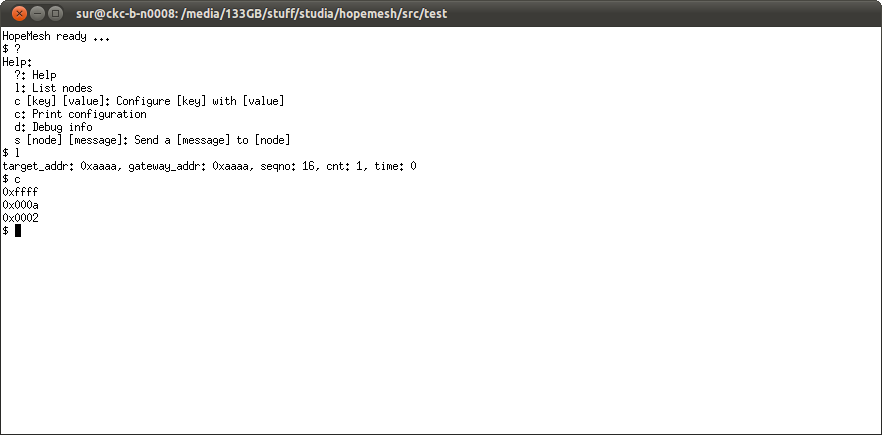
\includegraphics[width=\textwidth]{figures/research-shell1.png}
\caption{test-shell: The UART output screen}
\label{fig:test-shell1}
\end{figure}

Figure \ref{fig:test-shell2} shows the SPI output screen after issuing the command "\texttt{s 0xaaaa test}". Lines \texttt{000-001} show the byte stream from the RFM12B initialization routine. Lines \texttt{003-023} show the hamming byte stream as well as the sent raw packet stream.

\begin{figure}[H]
\centering
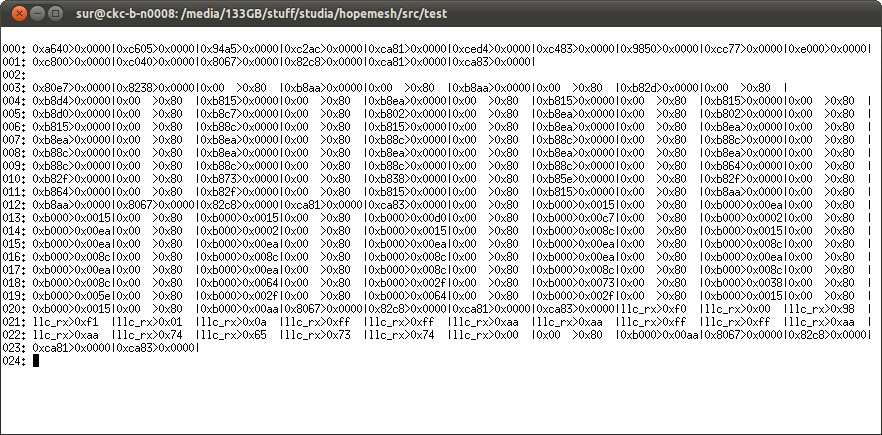
\includegraphics[width=\textwidth]{figures/research-shell2.png}
\caption{test-shell: The SPI output screen}
\label{fig:test-shell2}
\end{figure}

By using this data it can be easily verified that the sent packet byte stream includes the packet format from the previously defined network layers. Table \ref{tab:research_lowerlayers} shows the raw byte stream sent via SPI and table \ref{tab:research_llc} shows the hamming decoded byte stream. Both tables refer to the actual network layers.

\begin{table}[H]
\centering
\begin{tabular}{l | l | p{10cm}}
Bytes & Layer & Description \\
\hline
\texttt{0x80e7} & 1 & Enable the TX register (see \cite{sis4221_datasheet}) \\ 
\texttt{0x8238} & 1 & Enable the transceiver (see \cite{sis4221_datasheet}) \\ 
\texttt{0x00>0x80} & 1 & Status command 0x00, answer 0x80 = $10000000_{2}$ = RGIT (TX register is ready to receive the next byte) (see \cite{sis4221_datasheet}).

Now follow the send commands (0xb8) resembling the frame format from network layer 2a. \\ 
\texttt{0xb8aa} & 2a & AFC stabilizer pattern \\ 
\texttt{0xb8aa} & 2a & AFC stabilizer pattern \\ 
\texttt{0xb82d} & 2a & Sync pattern \\ 
\texttt{0xb8d4} & 2a & Sync pattern \\ 
\texttt{\dots} & 2b & Hamming encoded data\\ 
\texttt{0xb8aa} & 2a & Frame end \\ 
\texttt{0xb8aa} & 2a & Dummy byte \\ 
\texttt{0x8067} & 1 & Disable the TX register \\ 
\texttt{0x82c8} & 1 & Enable the receiver \\ 
\texttt{0xca81, 0xca83} & 1 & Reset the FIFO \\ 
\end{tabular}
\caption{Raw SPI byte stream}
\label{tab:research_lowerlayers}
\end{table}

\begin{table}[H]
\centering
\begin{tabular}{l | l | p{7cm}}
Bytes & Layer & Description \\
\hline
\texttt{0xf0 0x00} & 2b & The type 0x0 = $0_{10}$ and length 0xf = $15_{10}$ \\
\texttt{0x98 0xf1} & 2b & The CRC-16 checksum\\
\texttt{0x01 0xa} & 3 & The unicast version 0x1 = $1_{10}$ and TTL 0xa = $10_{10}$ \\
\texttt{0xff 0xff} & 3 & The originator address 0xffff \\
\texttt{0xaa 0xaa} & 3 & The target address 0xaaaa \\
\texttt{0xff 0xff} & 3 & The sender address 0xffff \\
\texttt{0xaa 0xaa} & 3 & The gateway address 0xaaaa \\
\texttt{0x74 0x65 0x73 0x74 0x00} & 4 & The ASCII encoded nul-terminated message string ("test") \\
\end{tabular}
\caption{Hamming decoded LLC byte stream}
\label{tab:research_llc}
\end{table}

\subsubsection{Conclusion} % {{{4
The above described research shows that:

\begin{itemize}
    \item The shell userspace module and UART driver module are working properly. They communicate correctly in the UART output screen, parse user input correctly and the described ring buffer algorithm reads and writes data in the correct order.
    \item The network library module and RFM12 driver module are working as expected and generate the correct frame and packet formats. The protocol used to communicate with the RFM12 radio module generates the correct commands.
\end{itemize}

\subsection{Routing}% {{{3
The next simulation emphasizes on the actual routing algorithm. Being the heart of the mesh communication it is very important to research whether the described algorithm as described in \ref{sub:route_propagation} is working correctly. For this purpose the author implemented a different simulation program which mainly simulates the network library module. It can be compiled by issuing the \texttt{make clean \&\& make test-batman} command in the \texttt{test} directory. After invoking the \texttt{test/test-batman} binary a total of 17 virtual experiments are executed and the results printed on the console. The next section will discuss each experiment and present the resulting simulated network topology.

\subsubsection{Test \#0}% {{{4
\begin{figure}[H]
  \begin{center}
    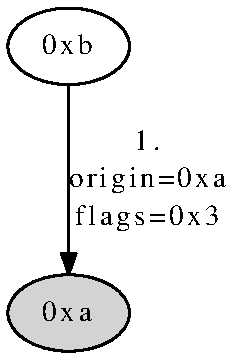
\includegraphics[]{figures/test0}
  \end{center}
  \caption{Route simulation test \#0}
  \label{fig:test0}
\end{figure}

The first test starts from the point of view of a single mesh node having the address \texttt{0xa}. All further operations are performed from this node. As can be seen in listing \ref{sim:test0} a rebroadcasted OGM originated by \texttt{0xa} itself sent from a direct neighbour \texttt{0xb} is being received. The corresponding topology is shown in figure \ref{fig:test0}.

\begin{lstlisting}[label=sim:test0,caption=Output of Test \#0]
rx:
llc: crc=0x0, len=8, type=1
ogm: sender_addr=0xb, originator_addr=0xa, flags=0x3, seqno=0, ttl=49

routing table: 
target_addr: 0xb, gateway_addr: 0xb, seqno: 0, cnt: 1, time: 0
\end{lstlisting}

The algorithm adds a new routing table to \texttt{0xb}. The \texttt{0xb} node rebroadcasted an OGM sent from \texttt{0xa} so we can be sure that \texttt{0xb} can hear him. From the point of view of \texttt{0xa} a bidirectional communication link exists. \texttt{0xb} additionally sets the unidirectional flag to indicate that he yet does not know whether \texttt{0xa} can hear him. \texttt{0xa} does not rebroadcast this OGM since it is targeted to him.

\subsubsection{Test \#1}% {{{4
\begin{figure}[H]
  \begin{center}
    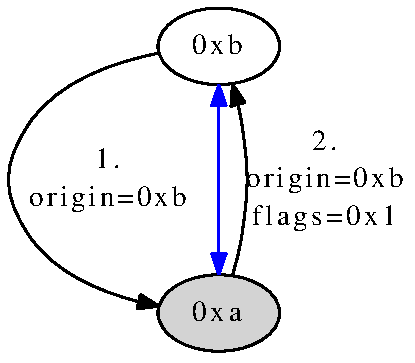
\includegraphics[]{figures/test1}
  \end{center}
  \caption{Route simulation test \#1}
  \label{fig:test1}
\end{figure}

Figure \ref{fig:test1} shows the updated network topology. The blue bidirectional arrow indicates our updated routing information to \texttt{0xb}. The second test now starts with the reception of an OGM originated by \texttt{0xb} and sent by him. Listing \ref{sim:test1} shows the algorithm behaviour.

\begin{lstlisting}[label=sim:test1,caption=Output of Test \#1]
rx:
llc: crc=0x0, len=8, type=1
ogm: sender_addr=0xb, originator_addr=0xb, flags=0x0, seqno=0, ttl=50

tx:
llc: crc=0x0, len=8, type=1
ogm: sender_addr=0xa, originator_addr=0xb, flags=0x1, seqno=0, ttl=49

routing table: 
target_addr: 0xb, gateway_addr: 0xb, seqno: 0, cnt: 2, time: 0
\end{lstlisting}

Node \texttt{0xa} rebroadcasts the received OGM from \texttt{0xb}. The TTL is being reduced by one and the "is direct" flag is set because \texttt{0xa} received this OGM from \texttt{0xb} directly. The unidirectional flag is not set because the link to \texttt{0xb} is assumed to be bidirectional.

\subsubsection{Test \#2}% {{{4
\begin{figure}[H]
  \begin{center}
    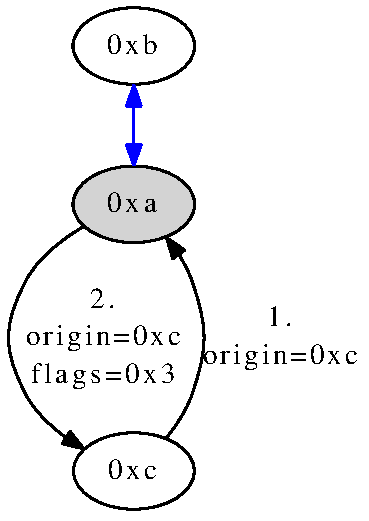
\includegraphics[]{figures/test2}
  \end{center}
  \caption{Route simulation test \#2}
  \label{fig:test2}
\end{figure}

The next test involves a new neighbour node \texttt{0xc} as shown in figure \ref{fig:test2}. It starts by receiving an OGM from \texttt{0xc} originated by him. Listing \ref{sim:test2} illustrates the algorithm behaviour.

\begin{lstlisting}[label=sim:test2,caption=Output of Test \#2]
rx:
llc: crc=0x0, len=8, type=1
ogm: sender_addr=0xc, originator_addr=0xc, flags=0x0, seqno=1, ttl=50

tx:
llc: crc=0x0, len=8, type=1
ogm: sender_addr=0xa, originator_addr=0xc, flags=0x3, seqno=1, ttl=49

routing table: 
target_addr: 0xb, gateway_addr: 0xb, seqno: 0, cnt: 2, time: 0
\end{lstlisting}

Node \texttt{0xa} rebroadcasts the received OGM from \texttt{0xc}. The "is direct" link is set as in the previous test but the unidirectional flag is set in contrast to the last test. No route entry to \texttt{0xc} is added since \texttt{0xa} has no confirmation about a bidirectional link from \texttt{0xc} yet.

\subsubsection{Test \#3}% {{{4
\begin{figure}[H]
  \begin{center}
    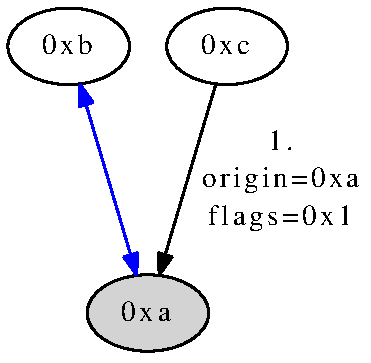
\includegraphics[]{figures/test3}
  \end{center}
  \caption{Route simulation test \#3}
\end{figure}

The next test starts with the reception of a rebroadcasted OGM sent from \texttt{0xc} originated by \texttt{0xa}. The "is direct" flag is set. Listing \ref{sim:test3} shows the algorithm behaviour.

\begin{lstlisting}[label=sim:test3,caption=Output of Test \#3]
rx:
llc: crc=0x0, len=8, type=1
ogm: sender_addr=0xc, originator_addr=0xa, flags=0x1, seqno=1, ttl=49

routing table: 
target_addr: 0xb, gateway_addr: 0xb, seqno: 0, cnt: 2, time: 0
target_addr: 0xc, gateway_addr: 0xc, seqno: 0, cnt: 1, time: 0
\end{lstlisting}

Node \texttt{0xc} is being added to the routing table and therefore a new direct bidirectional node neighbour. No OGM is being rebroadcasted since the received OGM is originated by \texttt{0xa}.

\subsubsection{Test \#4}% {{{4
\begin{figure}[H]
  \begin{center}
    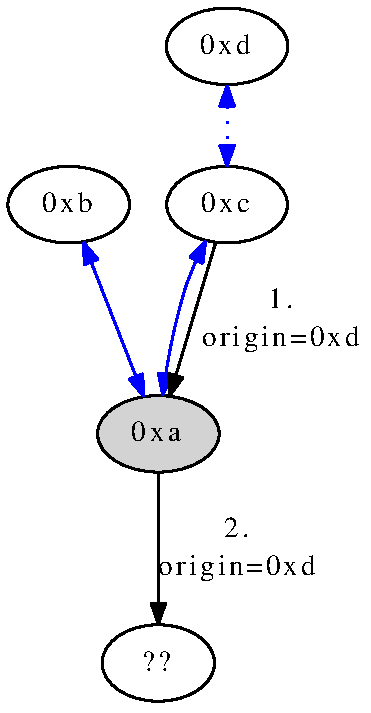
\includegraphics[]{figures/test4}
  \end{center}
  \caption{Route simulation test \#4}
\end{figure}

The next test starts with a rebroadcasted OGM sent from \texttt{0xc} (a direct bidirectional link neighbour) originated by \texttt{0xd}, an unknown node until now.

\begin{lstlisting}[label=sim:test1,caption=Output of Test \#4]
rx:
llc: crc=0x0, len=8, type=1
ogm: sender_addr=0xc, originator_addr=0xd, flags=0x0, seqno=23, ttl=49

tx:
llc: crc=0x0, len=8, type=1
ogm: sender_addr=0xa, originator_addr=0xd, flags=0x0, seqno=23, ttl=48

routing table: 
target_addr: 0xb, gateway_addr: 0xb, seqno: 0, cnt: 2, time: 0
target_addr: 0xc, gateway_addr: 0xc, seqno: 0, cnt: 1, time: 0
target_addr: 0xd, gateway_addr: 0xc, seqno: 23, cnt: 1, time: 0
\end{lstlisting}

Node \texttt{0xd} is being added to the route table. The gateway \texttt{0xc} is a know neighbour therefore a secure route can be persisted.

\subsubsection{Test \#5}% {{{4
\begin{figure}[H]
  \begin{center}
    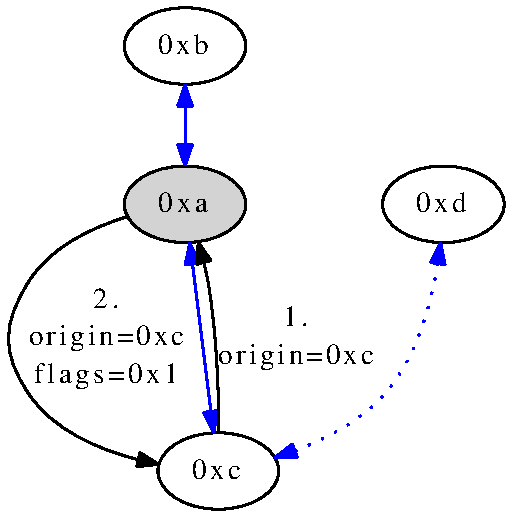
\includegraphics[]{figures/test5}
  \end{center}
  \caption{Route simulation test \#5}
\end{figure}

The next test shown in figure shows the reception of an OGM originated from \texttt{0xc}.

\begin{lstlisting}[label=sim:test1,caption=Output of Test \#5]
rx:
llc: crc=0x0, len=8, type=1
ogm: sender_addr=0xc, originator_addr=0xc, flags=0x0, seqno=1, ttl=50

tx:
llc: crc=0x0, len=8, type=1
ogm: sender_addr=0xa, originator_addr=0xc, flags=0x1, seqno=1, ttl=49

routing table: 
target_addr: 0xb, gateway_addr: 0xb, seqno: 0, cnt: 2, time: 0
target_addr: 0xc, gateway_addr: 0xc, seqno: 1, cnt: 2, time: 0
target_addr: 0xd, gateway_addr: 0xc, seqno: 23, cnt: 1, time: 0
\end{lstlisting}

As expected the OGM is being rebroadcasted by \texttt{0xa} with the "is direct" flag set.

\subsubsection{Tests \#6-\#9}% {{{4
\begin{figure}[H]
  \begin{center}
    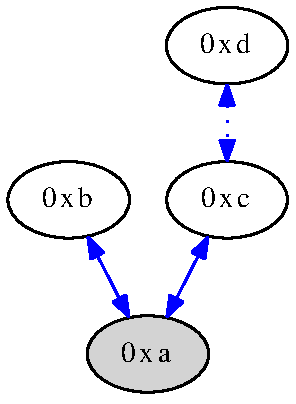
\includegraphics[]{figures/test6}
  \end{center}
  \caption{Route simulation test \#6-\#9}
  \label{fig:test6-9} 
\end{figure}

The next tests are based on the topology shown in figure \ref{fig:test6-9}. Since they are not of particular interest for the network topology (they test algorithmic corner-cases only) they are not further explained. The results can be inspected by executing the \texttt{test-batman} simulation.

\subsubsection{Test \#9}% {{{4
\begin{figure}[H]
  \begin{center}
    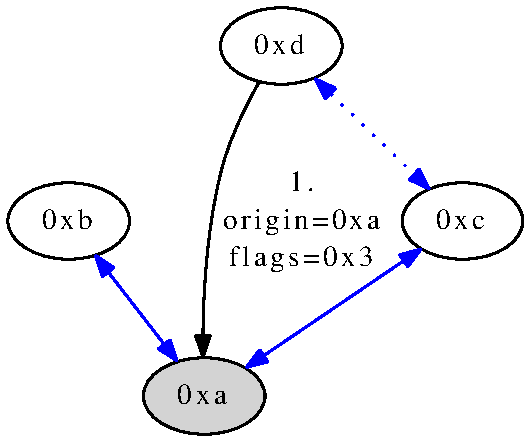
\includegraphics[]{figures/test9}
  \end{center}
  \caption{Route simulation test \#9}
\end{figure}

The next test brings a new interesting situation to node \texttt{0xa}. It now suddenly receives a direct OGM from \texttt{0xd} originated by \texttt{0xa}. \texttt{0xd} is already present in the route table via the gateway \texttt{0xc}. The behaviour of the algorithm is shown in the next listing.

\begin{lstlisting}[label=sim:test1,caption=Output of Test \#9]
rx:
llc: crc=0x0, len=8, type=1
ogm: sender_addr=0xd, originator_addr=0xa, flags=0x3, seqno=2, ttl=49

routing table: 
target_addr: 0xb, gateway_addr: 0xb, seqno: 0, cnt: 4, time: 0
target_addr: 0xc, gateway_addr: 0xc, seqno: 1, cnt: 2, time: 0
target_addr: 0xd, gateway_addr: 0xc, seqno: 23, cnt: 1, time: 0
target_addr: 0xd, gateway_addr: 0xd, seqno: 0, cnt: 1, time: 0
\end{lstlisting}

The node \texttt{0xd} is added as a direct bidirectional link neighbour because it rebroadcasted our own OGM. Note that we have now two route entries to node \texttt{0xd}, one direct link and one via the \texttt{0xc} gateway.

\subsubsection{Conclusion}% {{{4
\begin{figure}[H]
  \begin{center}
    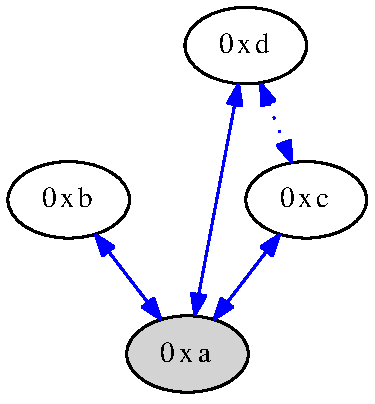
\includegraphics[]{figures/testfinal}
  \end{center}
  \caption{Final route simulation topology}
  \label{fig:testfinal}
\end{figure}

The final network topology is shown in figure \ref{fig:testfinal}. The tests \#10-\#12 only serve already presented cases (with different node addresses) so they are not discussed. The tests \#13-\#16 refer to unicast messages being evaluated based on the current route table and the assumed network topology in figure \ref{fig:testfinal}. Because unicast messages do not alter the network topology they are not further discussed.

The very last test \#17 shows what happens if after a time of simulated 16 seconds no OGM has been received. The result is an empty route table which implies a correct behaviour. Currently after 10 seconds a route entry must be deleted if no OGM was received in this timeout. Again the results can be inspected by invoking the \texttt{test-batman} program.

The research shows that the experiments based on a virtual simulation succeeded in a correct behaviour of the routing algorithm. Certainly not all cases of a network topology update were simulated but at least the basics of the algorithm work correctly.

\section{Mesh evaluation}% {{{2
probe \#1 \\
target\_addr: 0xb, gw\_addr: 0xb, seqno: 1000, lost: 4, cnt: 1000, time: 1038 \\
target\_addr: 0xa, gw\_addr: 0xa, seqno: 1000, lost: 10, cnt: 959, time: 963 \\

probe \#2 \\
target\_addr: 0xb, gw\_addr: 0xb, seqno: 1000, lost: 39, cnt: 982, time: 1056 \\
target\_addr: 0xa, gw\_addr: 0xa, seqno: 1050, lost: 10, cnt: 991, time: 995 \\

\chapter{Conclusion}% {{{1
\section{Open issues}% {{{2
Notes:\\
- Sequence numbers are ignored in the batman routing algorithm \\
- The transport layer is incomplete \\
- The MAC multiple access protocol can be much further improved\\
- The LLC layer does not split packets into frames and does not provide any means of flow control\\
- Sequence numbers are currently ignored for the routing metrics
- Larger number of mesh nodes


\begin{appendix}
\appendix
\chapter{CD content}
\label{chapter:appendix_a}
\begin{enumerate}
\item \textbf{src} --- The source files for the hopemesh implementation

\begin{itemize}
\item \textbf{ringbuf.c} --- The ringbuffer implementation
\end{itemize}

\end{enumerate}


\end{appendix}

\addcontentsline{toc}{chapter}{Literatura}
%\bibliographystyle{plain}
%\bibliographystyle{abbrv}
\bibliographystyle{is-unsrt}
\bibliography{bibliography}

\end{document}
